\documentclass[
12pt, % 字体大小
a4paper, 
oneside, % 单面打印(双面为twoside)
headinclude,footinclude, % 页眉页脚包含在文本区域内,确保不被裁剪或掩盖
]{scrartcl}
% 主题和样式
\usepackage[
nochapters, % 无章节层级 
beramono, % 等宽字体样式
eulermath, % 数学公式Euler字体
pdfspacing, % 字间距
dottedtoc % 点线式目录
]{classicthesis}
\usepackage{arsclassica} 
%----------------------------------------------------------------------------------------
% 输入和页面排版
\usepackage[T1]{fontenc} % 字体编码
\usepackage[utf8]{inputenc} % 输入编码
\usepackage{ctex} % 汉语
\usepackage{amsmath,amssymb,amsthm} % 数学公式
\usepackage{indentfirst} % 缩进
\setlength{\parindent}{2em} % 段落缩进
\usepackage[
top=2cm,
bottom=2cm, 
left=2cm,
right=2cm, 
headheight=20pt, 
includeheadfoot 
]{geometry} % 页面
\usepackage{scrlayer-scrpage} % 页眉页脚
\renewcommand{\sectionmark}[1]{\markright{\spacedlowsmallcaps{#1}}}
\renewcommand{\subsectionmark}[1]{\markright{\thesubsection~#1}}
\lehead{\mbox{\llap{\small\thepage\kern1em\color{halfgray} \vline}\color{halfgray}\hspace{0.5em}\rightmark\hfil}} % 标题旁边标记页码
\cfoot{\hyperlink{toc}{\color{RoyalBlue}返回目录}} % 页脚返回目录链接
\pagestyle{scrheadings}
%----------------------------------------------------------------------------------------
% 图表和引用
\usepackage{graphicx} % 图像
\graphicspath{{Figures/}} % 图像路径
\usepackage{subfig} % 图组
\usepackage{float} % 浮动
\usepackage{enumitem} % 列表
\usepackage{varioref} % 交叉引用
%----------------------------------------------------------------------------------------
% 代码
\usepackage{listings}
\lstset{
    language=Matlab,
    basicstyle=\ttfamily\small,   % 字体
    numbers=left,                 % 行号
    numberstyle=\tiny\color{gray},
    stepnumber=5,
    numbersep=5pt,
    backgroundcolor=\color{white},% 背景
    tabsize=2,                    % 制表符宽度
    frame=single,                 % 边框
    captionpos=t,                 % 标题
    title=\lstname,
    breaklines=true,              % 换行
    breakatwhitespace=true,
    escapeinside={`}{`},          % 转义(中文注释)
}
\lstset{
    language=Python,            
    basicstyle=\ttfamily\small,   % 字体
    numbers=left,                 % 行号
    numberstyle=\tiny\color{gray}, 
    stepnumber=5,             
    numbersep=5pt,            
    backgroundcolor=\color{white},% 背景
    tabsize=4,                    % 制表符宽度            
    frame=single,                 % 边框
    captionpos=t,                 % 标题
    title=\lstname, 
    breaklines=true,              % 换行
    breakatwhitespace=false,   
    escapeinside={`}{`},          % 转义(中文注释)
}
\usepackage{algorithm} % 算法
\usepackage{algpseudocode}
\usepackage{mdframed} % 跨页框架
% 不浮动算法环境
\newcounter{myalgorithm}
\renewcommand{\themyalgorithm}{\arabic{myalgorithm}}
\newenvironment{myalgorithm}[1][]{
  \refstepcounter{myalgorithm}
  \begin{mdframed}[
    skipabove=\topskip,
    skipbelow=\topskip,
    needspace=3\baselineskip,
    linewidth=0.4pt,
    frametitlefont=\normalfont\bfseries,
    frametitle={算法 \themyalgorithm\if\relax\detokenize{#1}\relax\else:#1\fi},
    frametitlerule=true,
    frametitlerulewidth=0.4pt,
    repeatframetitle=true
  ]
  \begin{algorithmic}[1]
  \ifx\relax\detokenize{#1}\relax
    \addcontentsline{alg}{algorithms}{\makebox[7em][l]{算法~\themyalgorithm} }
  \else
    \addcontentsline{alg}{algorithms}{\makebox[7em][l]{算法~\themyalgorithm} #1}
  \fi
}{
  \end{algorithmic}
  \end{mdframed}
}
% 关键词
\algrenewcommand{\algorithmicwhile}{当}
\algrenewcommand{\algorithmicdo}{执行}
\algrenewcommand{\algorithmicend}{结束}
\algrenewcommand{\algorithmicif}{如果}
\algrenewcommand{\algorithmicthen}{那么}
\algrenewcommand{\algorithmicelse}{否则}
\algrenewcommand{\algorithmicfor}{对于}
\algrenewcommand{\algorithmicrepeat}{循环}
\algrenewcommand{\algorithmicuntil}{直到}
\algrenewcommand{\algorithmicloop}{循环}
\algnotext{EndFor}
\algnotext{EndIf}
\algnotext{EndLoop}
\algnotext{EndWhile}
%----------------------------------------------------------------------------------------
% 超链接与PDF信息
\usepackage{hyperref} 
\hypersetup{
colorlinks=true, % 彩色
breaklinks=true, % 断行
urlcolor=webbrown, % URL棕色
linkcolor=RoyalBlue, % 内部链接蓝色
citecolor=webgreen, % 引用绿色
bookmarks=true, % 书签
bookmarksnumbered,
pdftitle={}, 
pdfauthor={},
pdfsubject={}, 
pdfkeywords={}, 
pdfcreator={pdfLaTeX}, 
pdfproducer={LaTeX with hyperref and ClassicThesis} 
}
%----------------------------------------------------------------------------------------
% 目录与标题
\usepackage{titlesec} 
\AtBeginDocument{
    \renewcommand{\contentsname}{目\hspace{1em}录}
    \renewcommand{\listfigurename}{图\hspace{1em}片}
    \renewcommand{\listtablename}{表\hspace{1em}格}
    \renewcommand{\figurename}{图}
    \renewcommand{\tablename}{表}
    \setcounter{tocdepth}{3} % 目录深度
}
\theoremstyle{definition} 
\newtheorem{definition}{定义}
\theoremstyle{plain} 
\newtheorem{theorem}{定理}
\theoremstyle{remark}
\newtheorem{remark}{备注}
\newtheorem{example}{样例}
\usepackage{tocloft} % 目录
% 要点目录
\newlistof{tips}{tip}{要\hspace{1em}点}
\newcommand{\tip}[1]{
  \refstepcounter{tips}
  \textsuperscript{\textcolor{orange}{\textbf{\thetips}}}
  \addcontentsline{tip}{tips}{\makebox[7em][l]{要点~\thetips} #1}
}
% 算法目录
\newlistof{algorithms}{alg}{算\hspace{1em}法} 
\hyphenation{Fortran hy-phen-ation} % 单词断字规则
%----------------------------------------------------------------------------------------
% 题目和作者
\title{\normalfont\spacedallcaps{强化学习}} 
\date{}
%----------------------------------------------------------------------------------------
% 开始和目录
\begin{document}
\maketitle
\newpage
\hypertarget{toc}{}
\begingroup
\begin{multicols}{2}
\tableofcontents
\end{multicols}
\endgroup
\newpage
\begingroup
\begin{multicols}{2}
\listoffigures
\end{multicols}
\endgroup
\hrule
\begingroup
\begin{multicols}{2}
\listoftables
\end{multicols}
\endgroup
\hrule
\begingroup
\begin{multicols}{2}
\listofalgorithms
\end{multicols}
\endgroup
\newpage
\listoftips
\newpage
%----------------------------------------------------------------------------------------
\section{导论}
%------------------------------------------------
\paragraph{特征}
智能体与环境交互(采样),在不断尝试中学习策略,使收益最大化。
\begin{itemize}
\item 试错探索:不会获知应采取的行动,通过尝试获得。
\item 延迟收益:一个动作的收益可能无法短期体现,而是长期浮现。
\item 环境不确定性:当前动作不但会影响当前收益,还会影响后续环境,进而影响后续收益。
\item 影响未知性:无法预测动作的影响,需要与环境频繁交互。
\item 试探(开拓动作空间)与开发/贪心(根据经验获得收益)折中。
\end{itemize}
%------------------------------------------------
\paragraph{优化方法对比}
\begin{itemize}
\item 凸优化:状态空间较小。可线性规划。
\item 最优控制:已知模型,解析回报函数。可动态规划,解HJB方程。
\item 进化算法:控制策略简单。如遗传算法。
\item 机器学习
\begin{itemize}
\item 有监督学习:有标签数据,注重推断与泛化能力。
\item 无监督学习:无标签数据,寻找数据隐含结构。
\end{itemize}
\item 强化学习:交互数据,优化策略以优化收益。
\end{itemize}
%------------------------------------------------
\paragraph{分类}
\begin{enumerate}
\item 模型依赖性
\begin{itemize}
\item 有模型:学习模型,规划策略。
\item 无模型:直接试错策略。
\end{itemize}
\item 策略更新方法
\begin{itemize}
\item 值函数:求解值函数重构策略。
\item 直接策略搜索:策略梯度等方法,搜索策略空间。
\item Actor-Critic方法:类似策略梯度,同时逼近值函数和策略。
\end{itemize}
\item 回报函数是否已知
\begin{itemize}
\item 正向:从回报到策略。
\item 逆向:从专家示例到回报。
\end{itemize}
\item 任务体量:分层强化学习、元强化学习、多智能体强化学习、迁移学习等
\item 框架
\begin{itemize}
\item 间接强化学习:充分利用有限经验,获得更好策略,减少与环境的交互。
\item 直接强化学习:不受模型设计偏差影响。
\end{itemize}
\end{enumerate}
%------------------------------------------------
\paragraph{发展}\label{sec:history back}~\\

值函数$ \rightarrow $直接策略搜索(策略梯度等)$ \rightarrow $深度强化学习。详见\ref{sec:history}。

发展方向:与深度学习结合,与专业知识结合,理论分析型增强,与认知科学结合,体量增大,与贝叶斯结合。
%----------------------------------------------------------------------------------------
\section{马尔可夫决策过程与贝尔曼方程}
%----------------------------------------------------------------------------------------
\subsection[马尔可夫决策过程]{马尔可夫决策过程(Markov decision process,MDP)}
%------------------------------------------------
\subsubsection[要素]{要素\tip{马尔可夫决策过程及其元素}}
\begin{itemize}
\item 状态(state,$ S $):强化学习依赖的概念。
\item 动作(action,$ A $):智能体做出的选择。
\item 奖励/收益(reward,$ R $):短期学习目标,环境给予智能体的信号。
\item 策略(policy,$ \pi $):在特定状态下,动作集的分布$ \pi(a|s) = p[A_t = a|S_t = s] $。
\item 回报(return,$ G $):长期收益累计,可能含有折扣,需综合评估。
\item 折扣因子($ \gamma \in [0, 1] $)。
\item 值函数(value function,$ V $):对$ s $预估的期望回报。
\item 行为/动作值函数($ Q $):对$ (s, a) $预估的期望回报。
\item 环境模型($ P $):模拟环境的反应,可以是确定性转移,也可以是随机性转移。
\item 大写字母表示空间,小写字母表示个体,上标$ ^* $表示最优。
\end{itemize}

\begin{figure}[H]
\centering 
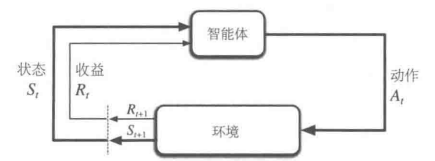
\includegraphics[width=0.5\textwidth]{Markov} 
\caption[马尔可夫决策过程]{马尔可夫决策过程}
\end{figure}
%------------------------------------------------
\subsubsection[状态、动作与收益]{状态、动作与收益}
%------------------------------------------------
\paragraph{序贯交互轨迹(trajectory)$ \tau =  s_0, a_0, r_1, s_1, a_1, r_2, \dots $}~\\

随机变量$ s',r $服从离散概率分布$ p(s', r|s, a) \doteq \Pr\{S_t = s', R_t = r|S_{t - 1} = s, A_{t - 1} = a\} $
$$ \sum_{s' \in S}\sum_{r \in R} p(s', r|s, a) = 1 $$。
%------------------------------------------------
\paragraph{马尔可夫性}\tip{马尔可夫性}
即“无记忆性”,未来状态仅依赖当前状态,而独立于过去状态。
$$ P(S_{t + 1}|S_t, S_{t - 1}, \dots, S_0) = P(S_{t + 1}|S_t) $$
%------------------------------------------------
\paragraph{状态转移与期望收益}~\\

由$ s $和$ a $转移到$ s' $的概率,包括$ s' $下各可能收益情况:
$$ p(s'|s, a) \doteq \Pr\{S_t = s'|S_{t - 1} = s, A_{t - 1} = a\} = \sum_{r \in R} p(s', r|s, a) $$

若不指定$ a $,由$ s $转移到$ s' $的概率为:
$$ p(s'|s) = \sum_{a \in A} [p(s'|s, a)p(a|s)] $$

有无$ s' $的两种期望收益:
\begin{align*}
r(s, a) &\doteq E[R_t|S_{t - 1} = s, A_{t - 1} = a] = \sum_{r \in R} r \sum_{s' \in S} p(s', r|s, a) \\
r(s, a, s') &\doteq E[R_t|S_{t - 1} = s, A_{t - 1} = a, S_t = s'] = \sum_{r \in R} r \frac{p(s', r|s, a)}{p(s'|s, a)}  
\end{align*}

\begin{figure}[H]
\centering
\subfloat[状态转移图(节点不能重复)]{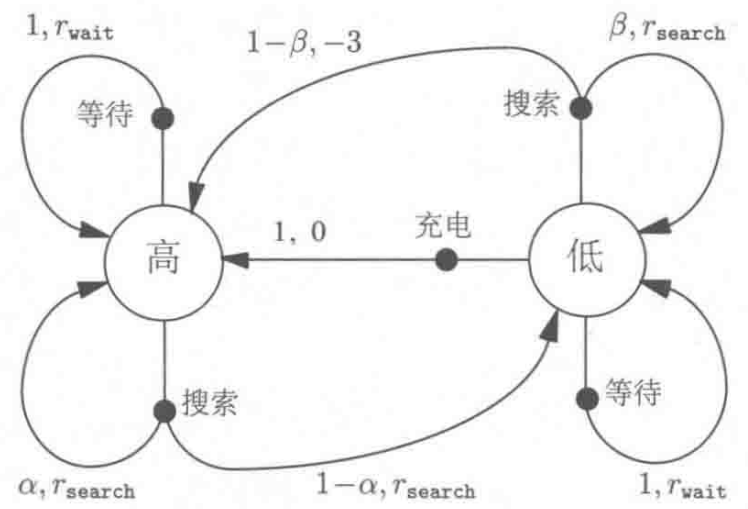
\includegraphics[width=.45\textwidth]{Transitions1}} \quad
\subfloat[状态转移表]{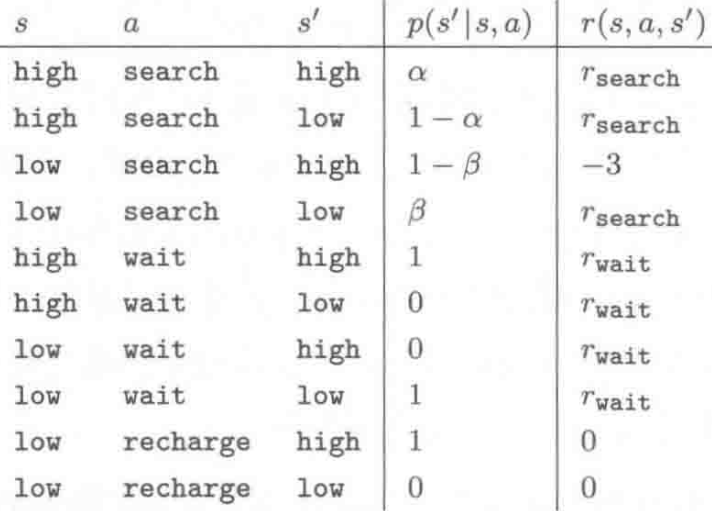
\includegraphics[width=.45\textwidth]{Transitions2}}
\caption[回收机器人状态转移]{回收机器人状态转移}
\end{figure}
%------------------------------------------------
\subsubsection[策略]{策略}
%------------------------------------------------
\paragraph{贪婪策略}
$ \pi(a|s) = argmax_a q(a) $。
%------------------------------------------------
\paragraph{探索-利用平衡策略}
\begin{itemize}
\item $ \epsilon $-greedy策略\tip{$ \epsilon $-greedy策略}:靠近贪心策略,但所有动作概率不为零。实际使用时需注意多最优情况。
$$
a = 
\begin{cases} 
argmax_a q(a) &, p = 1 - \epsilon \\
random(a) &, p = \epsilon
\end{cases}
\Rightarrow 
\pi(a|s) = 
\begin{cases} 
1 - \epsilon + \frac{\epsilon}{|A|} &, a = argmax_a q(a) \\
\frac{\epsilon}{|A|} &, otherwise
\end{cases}
$$
\item UCB(Upper Confidence Bound)策略:可以自适应平衡探索与利用。
$$ \pi(a|s) = Q(a) + c\sqrt{\frac{\ln N}{n(a)}} $$

其中,$ c $控制探索强度,$ N $是当前轮数,$ n(a) $是$ a $被选次数。
\item 玻尔兹曼分布(Boltzmann):可以动态调整探索强度。
$$ \pi(a|s) = \frac{e^{Q(a)/\tau}}{\sum_{a'} e^{Q(a)/\tau}} $$

其中$ \tau $是温度参数,控制随机程度,趋于$ 0 $时贪心,趋于$ \infty $时随机。
\item 高斯策略:
$$ \pi = \mu + \epsilon, \epsilon \sim N(0, \sigma^2) $$
\end{itemize}
%------------------------------------------------
\paragraph{增量式更新}\tip{增量式更新}
将轮次更新转化为递推关系,减少空间复杂度,如运行均值:
$$ Q_{n + 1} = \frac{1}{n}\sum_{i = 1}^n R_i = Q_n + \frac{1}{n}(R_n - Q_n) $$
%------------------------------------------------
\subsubsection[回报与折扣]{回报与折扣\tip{分幕与回报}}
\begin{itemize}
\item 幕(episode):一次交互序列,幕间没有联系。
\item 终止时刻$ T $:划分非终结状态集$ S $和所有状态集$ S^+ $。
\item 分幕式任务(episodic tasks):有终止状态,可分幕。
$$ G_t = R_{t + 1} + R_{t + 2} + \cdots + R_T = \sum_{k = t + 1}^T R_k $$
\item 持续性任务(continuing tasks):没有终止状态,持续进行,不能自然分幕。
$$ G_t = R_{t + 1} + \gamma R_{t + 2} + \gamma^2 R_{t + 3} + \cdots = \sum_{k = 0}^{\infty} \gamma^k R_{t + k + 1} \leq \frac{1}{1 - \gamma} max R_t $$

其中$ \gamma $越大代表长期收益越重要。
\item 统一表示:有限项终止后,状态持续转移回自己,相当于无限项。
$$ G_t \doteq \sum_{k = t + 1}^{T} \gamma^{k - t - 1} R_k $$
\end{itemize}
%------------------------------------------------
\subsubsection[值函数]{值函数\tip{值函数与回溯算法}}
%------------------------------------------------
\paragraph{值函数}
\begin{align*}
v_\pi(s) &\doteq E_\pi[G_t|S_t = s] = E_\pi[\sum_{k = 0}^{\infty} \gamma^k R_{t + k + 1}|S_t = s], s \in S \\
&= E_\pi[\underbrace{R_{t + 1}}_{\text{即时奖励}} + \gamma \underbrace{G_{t + 1}}_{\text{未来奖励}}|S_t = s] (\text{后继递推关系}) \\
&= \sum_{a \in A} \pi(a|s)[\sum_{r \in R} p(r|s, a)r + \gamma \sum_{s' \in S} p(s'|s, a)v_{\pi}(s')] (\text{分项全概率展开}) \\
&= \underbrace{\sum_{a \in A} \pi(a|s) \overbrace{\sum_{s' \in S, r \in R} p(s', r|s, a)[r + \gamma v_\pi(s')]}^{q_{\pi}(s, a)}}_{\text{贝尔曼方程}} (\text{值函数递推关系})
\end{align*}
%------------------------------------------------
\paragraph{行为值函数}
\begin{align*} 
q_\pi(s, a) &\doteq E_\pi[G_t|S_t = s, A_t = a] = E_\pi[\sum_{k = 0}^{\infty} \gamma^k R_{t + k + 1}|S_t = s, A_t = a], s \in S \\
&= \sum_{r \in R} p(r|s, a)r + \gamma \sum_{s' \in S} P(s'|s, a) \underbrace{\sum_{a' \in A} \pi(a'|s')q_{\pi}(s'|a')}_{v_{\pi}(s')} (\text{状态值函数递推关系})
\end{align*}
%------------------------------------------------
\paragraph{回溯算法}
$ s' $的价值信息回传给$ s $。

\begin{figure}[H]
\centering 
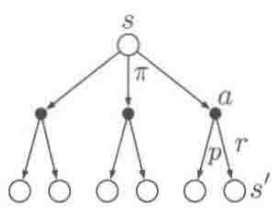
\includegraphics[width=0.25\textwidth]{DP} 
\caption[DP回溯图]{DP回溯图(节点可以重复)}
\end{figure}
%------------------------------------------------
\paragraph{最优值函数与最优策略}
\begin{itemize}
\item $ \forall s \in S, q_{\pi}(s, \pi'(s)) = v_{\pi'}(s) \geq v_{\pi}(s) $,则称$ \pi' $优于或等于$ \pi $。
\item $ v_\pi(s) $定义了$ \pi $的偏序关系,$ \pi^* $存在且可能不唯一,它们共享:
$$ v^*(s) \doteq \max_{\pi} v_{\pi}(s) \quad q^*(s, a) \doteq \max_{\pi} q_{\pi}(s, a) $$
\end{itemize}
%------------------------------------------------
\subsubsection[构建要点]{构建要点}
\begin{itemize}
\item 确定$ s,a,r $(不含先验知识,不为达到子目标而舍弃最终目标)。
\item 奖励与惩罚是相对的,可以全奖励或全惩罚。
\item 同一问题可能有多层次MDP。
\item 利用先验知识,人为排除愚蠢动作。
\end{itemize}
%----------------------------------------------------------------------------------------
\subsection[贝尔曼方程]{贝尔曼方程\tip{贝尔曼方程}}
%------------------------------------------------
\subsubsection[贝尔曼方程]{贝尔曼方程}
\begin{align*}
\underline{v_\pi(s)} &= \sum_{a \in A} \pi(a|s) \sum_{s' \in S, r \in R} P(s', r|s, a)[r + \gamma \underline{v_\pi(s')}] \\
&= \underbrace{\sum_{a \in A} \pi(a|s) \sum_{r \in R} P(r|s, a)}_{r_{\pi}(s)} + \gamma \sum_{s' \in S} [\underbrace{\sum_{a \in A} \pi(a|s)P(s'|s, a)}_{p_{\pi}(s'|s)}] \underline{v_\pi(s')} 
\end{align*}
%------------------------------------------------
\subsubsection[贝尔曼最优方程]{贝尔曼最优方程}
方程组中方程数为$ |S| $,如$ P $已知,并具有马尔可夫性,则可求解。但一般难以满足,且计算资源有限,求近似解。
%------------------------------------------------
\paragraph{形式}
\begin{itemize}
\item $ s \rightarrow a^* $:
\begin{align*}
v^*(s) &= \max_{a \in A} q_{\pi^*}(s, a) (\text{凸组合最优}) \\
&= \max_{\pi} \sum_{s \in S} \pi(a|s)q(s,a) (\text{元素}) \\
&= \max_{\pi} (r_\pi + \gamma P_\pi v) (\text{矩阵})
\end{align*}
\item $ (s, a) \rightarrow (s, a)_{next}^* $:
\begin{align*}
q^*(s, a) &= E[R_{t + 1} + \gamma \max_{a'} q^*(S_{t + 1}, a')|S_t = s, A_t = a] \\
&= \sum_{s' \in S, r \in R} p(s', r|s, a)[r + \gamma \max_{a'} q^*(s', a')]
\end{align*}
\end{itemize}

\begin{figure}[H]
\centering 
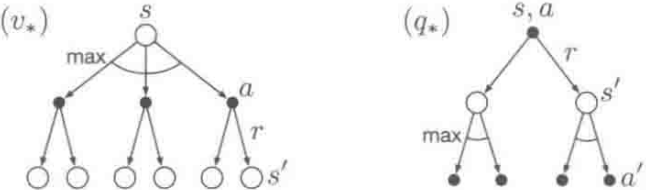
\includegraphics[width=0.7\textwidth]{DPbest} 
\caption[DP回溯图的两种形式(最优)]{DP回溯图的两种形式(最优)}
\end{figure}
%------------------------------------------------
\paragraph{求解}\label{sec:Scalability Mapping back}
伸缩映射性,见\ref{sec:Scalability Mapping}。
%------------------------------------------------
\paragraph{贪婪最优策略}
$ \pi^* $中,$ v(s) = E[r(a^*|s)] $,可使用贪心策略求取(证明:凸组合最大值为最大一项)。
%----------------------------------------------------------------------------------------
\section[动态规划]{动态规划(Dynamic Programming,DP):期望更新}
\begin{minipage}{0.5\textwidth}
\hspace{2em}
使用值函数结构化组织最优策略搜索,将贝尔曼方程转化成近似逼近理想值函数的递归更新公式,即将多阶段决策问题转化为多个单阶段决策问题。
\end{minipage}
\hfill
\begin{minipage}{0.45\textwidth}
\begin{figure}[H]
\centering 
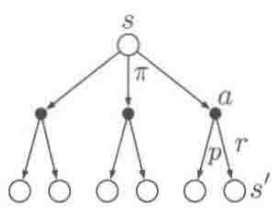
\includegraphics[width=0.6\textwidth]{DP} 
\caption[DP回溯图]{DP回溯图:显示一步的所有转移}
\end{figure}
\end{minipage}
%------------------------------------------------
\subsection[策略迭代]{策略迭代\tip{策略迭代}}
$$ \pi_0 \xrightarrow{PE} v_{\pi_0} \xrightarrow{PI} \pi_1 \xrightarrow{PE} v_{\pi_1} \xrightarrow{PI} \pi_2 \xrightarrow{PE} v_{\pi_2} \xrightarrow{PI} \dots $$

反复进行PE和PI,得到改进的$ v_{\pi} $估计和$ \pi $,最后收敛到最优。
\begin{itemize}
\item 策略评估(PE):
\begin{itemize}
\item 直接求解:$ v_{\pi_k} = (I - \gamma P_{\pi_k})^{-1} r_{\pi_k} $。
\item 迭代求解:
$$ \underbrace{v_{\pi_k}^{(j + 1)} = r_{\pi_k} + \gamma P_{\pi_k} v_{\pi_k}^{(j)} = \sum_{a \in A} \pi(a|s)[r(a|s) + \gamma \sum_{s' \in S}P(s'|s, a)v_{\pi}(s')], j = 0, 1, 2, \dots}_{\text{期望更新:基于后继可能状态的期望值}} $$
\item 截断策略评估:不需要完全收敛。
\end{itemize}
\item 策略改进(PI):
\begin{itemize}
\item 理论:$ v_{\pi}(s) \leq q_{\pi}[s, \pi'(s)] $则$ \pi' $不次于$ \pi $
\begin{align*}
v_{\pi}(s) &\leq q_{\pi}[s, \pi'(s)] \\
&= E_{\pi'} [R_{t + 1} + \gamma v_{\pi}(S_{t + 1})|S_t = s, A_t = \pi'(s)] \\
&\leq E_{\pi'} \{R_{t + 1} + \gamma q_{\pi}[S_{t + 1}, \pi'(S_{t + 1})]|s_t = s\} \\
&\leq E_{\pi'} [R_{t + 1} + \gamma R_{t + 2} + \gamma^2 R_{t + 3} + \dots|S_t = s] \\
&= v_{\pi'}(s)
\end{align*}
\item 贪心策略:$ \pi_{k + 1} = argmax_{\pi}(r_{\pi} + \gamma P_{\pi} v_{\pi_k}) $
\end{itemize}
\end{itemize}
%------------------------------------------------
\begin{myalgorithm}[策略迭代]
\State 参数:估计精度阈值$ \theta > 0 $
\State 初始化:$ \forall s \in S $,任意初始化$ v(s) \in R, \pi(s) $
\Repeat
\Repeat \Comment{策略评估}
\State $ \Delta \gets 0 $
\For{$ \forall s \in S $}
\State $ v_{\pi_k}^{(j + 1)}(s) \gets \sum_{a \in A} \pi_k(a|s)[\sum_{r \in R} p(r|s,a)r + \gamma \sum_{s' \in S} p(s'|s,a) v_{\pi_k}^{(j)}(s')] $
\State $ \Delta \gets \max(\Delta, |v - v_{\pi_k}^{(j + 1)}(s)|) $
\EndFor
\Until{$ \Delta < \theta $}
\State 策略稳定$ \gets $true \Comment{策略改进}
\For{$ \forall s \in S $}
\State $ a_{old} \gets \pi(s) $
\For{$ \forall a \in A(s) $}
\State $ q_{\pi_k}(s, a) \gets \sum_{r \in R} p(r|s, a)r + \gamma \sum_{s' \in S} p(s'|s, a)v_{\pi_k}(s') $
\EndFor
\State $ a^*_k(s) \gets argmax_a q_{\pi_k}(s, a) $,并更新$ \pi(s)  $
\If{$ a_{old} \neq a^*_k(s) $}
\State 策略稳定$ \gets $false
\EndIf
\EndFor
\Until{策略稳定}
\end{myalgorithm}
%------------------------------------------------
\subsection[值迭代]{值迭代\tip{值迭代}}
$$ u_0 \xrightarrow{PU} \pi'_1 \xrightarrow{VU} u_1 \xrightarrow{PU} \pi'_2 \xrightarrow{VU} u_2 \xrightarrow{PU} \dots $$

结合极端PE和PI,只进行一次PE遍历,对每个状态更新一次。
$$ v_{k + 1} = \max_{\pi} r_{\pi} + \gamma P_{\pi}v_k, k = 1, 2, 3, \dots $$
\begin{itemize}
\item 策略更新(PU):$ \pi_{k + 1} = argmax_{\pi}(r_{\pi} + \gamma P_{\pi}v_k) $,贪婪选取。
\item 价值更新(VU):$ v_{k + 1} = r_{\pi_{k + 1}} + \gamma P_{\pi_{k + 1}}v_k = max_{a \in A} q_k $。
\end{itemize}
%------------------------------------------------
\begin{myalgorithm}[值迭代]
\State 参数:估计精度阈值$ \theta > 0 $
\State 初始化:$ \forall s \in S^+ $,任意初始化$ v(s), v(\text{终止}) = 0 $
\Repeat
\State $ \Delta \gets 0 $
\For{$ \forall s \in S $}
\For{$ \forall a \in A(s) $}
\State $ q_k(s, a) \gets \sum_{r \in R} p(r|s, a)r + \gamma \sum_{s' \in S} p(s'|s, a)v_k(s') $
\State $ a^*_k(s) \gets argmax_a q_k(s, a) $ \Comment{贪婪策略}
\State 若$ a = a^*_k $且$ \pi_{k + 1}(a|s) = 0 $,则令$ \pi_{k + 1}(a|s) = 1 $ \Comment{策略更新}
\State $ v_{k + 1}(s) \gets \max_a q_k(s, a) $ \Comment{价值更新}
\State $ \Delta \gets \max(\Delta, |v_{k + 1} - v_k|) $ \Comment{一轮中反复更新精度}
\EndFor
\EndFor
\Until{$ \Delta < \theta $}
\end{myalgorithm}
%------------------------------------------------
\subsection[对比与补充]{对比与补充}\label{sec:DP back}
\begin{table}[H]
\centering
\caption{DP对比}
\begin{tabular}{|c|c|c|}
\hline
& 策略迭代 & 值迭代 \\
\hline
维护内容 & 值函数+策略 & 值函数 \\
\hline
收敛速度 & 较快 & 较慢 \\
\hline
收敛性 & 依赖初始策略质量,可能陷入局部最优 & 保证全局最优 \\
\hline
适用策略空间 & 简单 & 复杂 \\
\hline
计算成本 & 较低 & 较高(迭代遍历所有动作) \\
\hline
\end{tabular}
\end{table}

补充见\ref{sec:DP}。
%----------------------------------------------------------------------------------------
\section[蒙特卡洛]{蒙特卡洛(Monte Carlo,MC):采样更新}
针对分幕式任务,不需要$ P $,通过多幕采样数据获得经验代替值函数解决问题。
%------------------------------------------------
\subsection[概念]{概念\tip{蒙特卡洛}}
%------------------------------------------------
\paragraph{核心需求}
由于$ P $的缺失,$ v(s) $是不够的,需要评估$ q(s, a) $。
%------------------------------------------------
\paragraph{估计$ q(s, a) $}
\begin{itemize}
\item 访问(visit):给定的一幕中,指定状态的一次出现。
\item 首次访问(first visit):$ \hat{q}(s, a) = \frac{G_{11}(s, a) + G_{21}(s, a) + \dots}{N(s, a)} $。
\item 每次访问(every visit):$ \hat{q}(s, a) = \frac{G_{11}(s, a) + G_{12}(s, a) + \dots + G_{21}(s, a) + \dots}{N(s, a)} $。
\end{itemize}

$ N(s) $是$ s $的访问次数,$ N(s) \to \infty, \hat{q}(s, a) \to q_{\pi}(s, a) $。

\begin{figure}[H]
\centering 
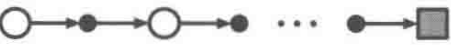
\includegraphics[width=0.3\textwidth]{MC} 
\caption[MC回溯图:显示一幕所有采样到的转移]{MC回溯图:显示一幕所有采样到的转移}
\end{figure}
%------------------------------------------------
\paragraph{幕长}
靠近目标的状态比远离目标的状态更早具有非零值,幕长应足够长,无需无限长。
%------------------------------------------------
\paragraph{优势}
\begin{itemize}
\item 不需要$ P $,可从实际经历和模拟经历中学习。
\item 对每个状态的估计是独立的,可聚焦于状态子集,无需考虑其他状态,效率高。
\item 无马尔可夫性时性能损失较小。
\end{itemize}
%------------------------------------------------
\paragraph{恒温策略:$ \forall(s, a), \pi(a|s) > 0 $}
\begin{enumerate}
\item 试探性出发(ES):为采样部分无法正常获得的$ (s, a) $,可设定所有$ (s, a) $都有概率作为起始。满足充分探索的理论要求,但实际中很难实现。
\item $ \epsilon $-greedy策略。
\end{enumerate}
%------------------------------------------------
\subsection[on-policy]{on-policy(同轨)\tip{on-policy}}
采样并改进相同策略。
%------------------------------------------------
\begin{myalgorithm}[MC-On-policy(first visit)]
\State 参数:$ \epsilon > 0 $
\State 初始化:$ \forall s \in S, a \in A(s) $,任意初始化$ q(s,a) \in R $,初始化$ Returns(s,a) $为空列表,$ \epsilon $-greedy初始化$ \pi $
\Loop
\State 根据$ \pi $生成一幕序列$ S_0, A_0, R_1, S_1, A_1, R_2, \dots, S_{T - 1}, A_{T - 1}, R_T $
\State $ G \gets 0 $
\For{$ t = T - 1, T - 2, \dots, 0 $}
\State $ G \gets \gamma G + R_{t + 1} $
\If{$ S_t $在此幕中首次出现}
\State 将$ G $加入$ Returns(S_t,A_t) $
\State $ q(S_t, A_t) \gets average[Returns(S_t, A_t)] $
\State $ a^* \gets argmax_a q(S_t, a) $
\State $ \epsilon $-greedy策略选取$ \pi(a|S_t) $
\EndIf
\EndFor
\EndLoop
\end{myalgorithm}
%------------------------------------------------
\subsection[off-policy]{off-policy(离轨)\tip{off-policy}}
采样与改进不同策略,前者称为行为策略(Behavior Policy)$ b $(保证对所有可能动作的采样),后者称为目标策略(Target Policy)$ \pi $。
%------------------------------------------------
\paragraph{重要度采样(importance sampling)}\tip{重要度采样}\label{sec:MC back}
计算$ G $时,对轨迹在$ \pi $和$ b $中出现的相对概率进行加权:
$$ \rho_{t:T - 1} = \Pi_{k = t}^{T - 1} \frac{\pi(A_k|S_k)}{b(A_k|S_k)} (\text{约去相同的转移概率}) $$
\begin{itemize}
\item 普通重要度采样:$ v(s) \doteq \frac{\sum_{t \in \tau(s)} \rho_{t:T(t) - 1}G_t}{|\tau(s)|} $,无偏但无界。
\item 加权重要度采样:$ v(s) \doteq \frac{\sum_{t \in \tau(s)} \rho_{t:T(t) - 1}G_t}{\sum_{t \in \tau(s)} \rho_{t:T(t) - 1}} $,有偏但偏差值渐近收敛。
\end{itemize}

减小方差的方法见\ref{sec:MC}。
%------------------------------------------------
\paragraph{增量式更新}
\begin{align*}
v_{n + 1} &\doteq v_n + \frac{W_n}{C_n}[G_n - v_n] (v_n \text{和} G_n \text{线性组合}) \\
C_{n + 1} &\doteq C_n + W_{n + 1}
\end{align*}

其中,$ W_i $是随机权重,$ C_i $是其累加和。
%------------------------------------------------
\begin{myalgorithm}[MC-Off-policy(every visit)]
\State 初始化:$ \forall s \in S, a \in A(s) $,任意初始化$ q(s,a) \in R, C(s,a) = 0 $,初始化$ \pi(s) = argmax_a q(s,a) $ \Comment{目标策略为贪婪策略}
\Loop
\State 根据$ b $生成一幕序列$ S_0, A_0, R_1, S_1, A_1, R_2, \dots, S_{T - 1}, A_{T - 1}, R_T $ \Comment{行为策略为$ \epsilon $-greedy策略}
\State $ G \gets 0, W \gets 1 $
\For{$ t = T - 1, T - 2, \dots, 0 $}
\State $ G \gets \gamma G + R_{t + 1} $
\State $ C(S_t, A_t) \gets C(S_t, A_t) + W $
\State $ q(S_t ,A_t) \gets q(S_t, A_t) + \frac{W}{C(S_t, A_t)}[G - q(S_t, A_t)] $ \Comment{增量式更新}
\State $ \pi(S_t) \gets argmax_a q(S_t,a) $
\If{$ A_t \neq \pi(S_t) $}
\State break \Comment{如果不是最优动作则退出内层循环}
\EndIf
\State $ W \gets \frac{W}{b(A_t|S_t)} $ \Comment{更新重要度采样权重}
\EndFor
\EndLoop
\end{myalgorithm}

潜在问题:贪心行为普遍时,只会从幕尾学习;贪心行为不普遍时,学习速度较慢。
%------------------------------------------------
\subsection[对比]{对比}
\begin{table}[H]
\centering
\caption{MC对比}
\begin{tabular}{|c|c|c|}
\hline
策略类型 & 稳定性 & 收敛性 \\
\hline
on-policy & 较稳定 & 需要更多样本(更新需要新的数据) \\
\hline
off-policy & 不太稳定(使用行为策略) & 更快找到优质解 \\
\hline
\end{tabular}
\end{table}
%----------------------------------------------------------------------------------------
\section[时序差分]{时序差分(Temporal Difference,TD):采样更新}
TD可直接从与环境的互动中获取信息,不需要$ P $,同时运用自举思想,可基于已得到的其他状态估计来更新当前$ v(s) $,相当于结合了DP和MC的优点。
%------------------------------------------------
\subsection[TD($ 0 $)]{TD($ 0 $)\tip{时序差分(TD($ 0 $))}}
更新公式为:
$$ v_{t + 1}(s_t) = v_t(s_t) + \alpha_t(s_t)[\overbrace{\underbrace{r_{t + 1} + \gamma v_t(s_{t + 1})}_{\text{TD目标(target)}} - v_t(s_t)}^{\text{新息:TD误差(error)}\delta_t}] $$

\begin{itemize}
\item $ G_t $是$ v_{\pi}(s_t) $的无偏估计;$ r_{t + 1} + \gamma v_{\pi}(s_{t + 1}) $是无偏估计,而$ r_{t + 1} + \gamma v(s_{t + 1}) $是有偏估计。
\item MC误差可写成TD误差之和$ G_t - v(s_t) = \sum_{k = t}^{T - 1} \gamma^{k - t} \delta_k $,其在步长较小时成立。
\end{itemize}

\begin{figure}[H]
\centering
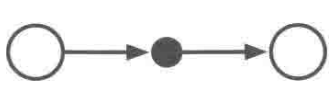
\includegraphics[width=0.2\textwidth]{TD}
\caption[TD回溯图]{TD回溯图}
\end{figure}
%------------------------------------------------
\paragraph{优势}
\begin{itemize}
\item 不需要$ P,R $。
\item 更新快:MC须等到幕尾确定增量,更新$ G_t $;而TD只需等到下一时刻,更新TD目标。
\item 方差小:MC更新依赖很多随机动作,TD更新仅依赖一个随机动作,因此TD目标的方差比$ G_t $的方差要小很多。
\item 随机任务中,TD($ 0 $)收敛速度要比常量$ \alpha $MC快。前者的最优性与预测回报更相关,找出的是完全符合马尔可夫过程的最大似然估计参数,收敛到确定性等价估计;而后者只在有限方面最优,找出的是最小化训练集均方误差的估计。
\item 自举性:TD需要初始猜测值,MC没有进行初始猜测。
\item 只评估当前动作,与后续动作无关。
\end{itemize}
%------------------------------------------------
\begin{myalgorithm}[TD($ 0 $)]
\State 输入:待评估策略$ \pi $
\State 参数:步长$ \alpha \in (0, 1] $
\State 初始化:$ \forall s \in S^+ $,任意初始化$ v(s), v(\text{终止}) = 0 $
\For{每一幕}
\State 初始化$ s $
\While{$ s $不是终止状态}
\State 由$ \pi(s) $获得$ a $并执行,观察$ r, s' $
\State $ v(s) \gets v(s) + \alpha[r + \gamma v(s') - v(s)] $
\State $ s \gets s' $
\EndWhile
\EndFor
\end{myalgorithm}
%------------------------------------------------
\subsection[Sarsa]{Sarsa(on-policy-TD)\tip{Sarsa(on-policy-TD)}}
Sarsa(State-Action-Reward-State-Action),更新单元为$ (s_t, a_t, r_t, s_{t + 1}, a_{t + 1}) $,是TD算法的$ q(s, a) $版本:
$$ q_{t + 1}(s_t, a_t) = q_t(s_t, a_t) + \alpha_t(s_t, a_t)[r_{t + 1} + \gamma q_t(s_{t + 1}, a_{t + 1}) - q_t(s_t, a_t)] $$

\begin{figure}[H]
\centering
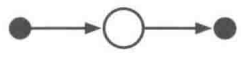
\includegraphics[width=0.2\textwidth]{Sarsa}
\caption[Sarsa回溯图]{Sarsa回溯图}
\end{figure}
%------------------------------------------------
\begin{myalgorithm}[Sarsa(on-policy-TD)]
\State 参数:步长$ \alpha \in (0,1], \epsilon > 0 $
\State 初始化:$ \forall s \in S^+ $,任意初始化$ q(s,a), q(\text{终止}, \cdot) = 0 $
\For{每一幕}
\State 初始化$ s $
\State 使用从$ q $得到的$ \epsilon $-greedy策略,在$ s $选择$ a $
\While{$ s $不是终止状态}
\State 执行$ a $,观察$ r, s' $
\State 使用从$ q $得到的$ \epsilon$-greedy策略,在$ s' $处选择$ a' $
\State $ q(s, a) \gets q(s, a) + \alpha [R + \gamma q(s', a') - q(s, a)] $
\State $ s \gets s', a \gets a' $
\EndWhile
\EndFor
\end{myalgorithm}
%------------------------------------------------
\paragraph{期望Sarsa}
$$ q_{t + 1}(s_t, a_t) = q_t(s_t, a_t) + \alpha_t(s_t, a_t)\{r_{t + 1} + \gamma[\underbrace{\sum_a \pi(a|s_{t + 1}) q_t(s_{t + 1}, a)}_{v_t(s_{t + 1})}] - q_t(s_t, a_t)\} $$

\begin{minipage}{0.6\textwidth}
\begin{itemize}
\item 相较Sarsa,期望Sarsa虽然计算复杂,但消除了随机选择带来的方差。
\item $ \alpha $的选择会影响长期稳态性等指标。
\item 生成策略可以基于相同或不同策略,即离轨或在轨是可变的,因此Q-learning可视为期望Sarsa的特例。
\end{itemize}
\end{minipage}
\hfill
\begin{minipage}{0.35\textwidth}
\begin{figure}[H]
\centering
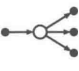
\includegraphics[width=0.5\textwidth]{eSarsa}
\caption[期望Sarsa回溯图]{期望Sarsa回溯图}
\end{figure}
\end{minipage}
%------------------------------------------------
\subsection[Q-learning]{Q-learning(off-policy-TD)\tip{Q-learning(off-policy-TD)}}
Q-learning旨在求解行为值贝尔曼最优方程,直接逼近$ q^*(s, a) $,更新单元为$ (s_t, a_t, r_t, s_{t + 1}) $。
$$ q_{t + 1}(s_t, a_t) = q_t(s_t, a_t) + \alpha_t(s_t, a_t)[r_{t + 1} + \gamma \max_a q_t(s_{t + 1}, a) - q_t(s_t, a_t)] $$

\begin{figure}[H]
\centering
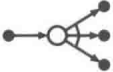
\includegraphics[width=0.2\textwidth]{Q}
\caption[Q-learning回溯图]{Q-learning回溯图}
\end{figure}
%------------------------------------------------
\begin{myalgorithm}[Q-learning(off-policy-TD)]
\State 参数:步长$ \alpha \in (0,1] $,探索率$ \epsilon > 0 $
\State 初始化:$ \forall s \in S^+, a \in A(s) $,任意初始化$ q(s,a), q(\text{终止}, \cdot) = 0 $
\For{每一幕}
\State 初始化$ s $
\While{$ s $不是终止状态}
\State 使用从$ q $得到的$ \epsilon $-greedy策略,在$ s $选择$ a $并执行,观察$ r, s' $
\State $ q(s, a) \gets q(s, a) + \alpha [r + \gamma \max_a q(s', a) - q(s, a)] $
\State $ s \gets s' $
\EndWhile
\EndFor
\end{myalgorithm}
%------------------------------------------------
\paragraph{双Q-learning}
双学习:划分样本,学习两个独立的估计$ q_1(a), q_2(a) $,确定$ a^* = argmax_a q_1(a) $,再计算$ q_2(a*) = q_2(argmax_a q_1(a)) $,后者是无偏的(可以交换再来一次)。需要双倍内存,但是计算量不会增大。
$$ q_{1_{t + 1}}(s_t, a_t) = q_{1_t}(s_t, a_t) + \alpha_t(s_t, a_t)\{r_{t + 1} + \gamma q_{2_t}[s_{t + 1}, argmax_a q_{1_t}(s_{t + 1}, a)] - q_{1_t}(s_t, a_t)\} $$

\begin{figure}[H]
\centering
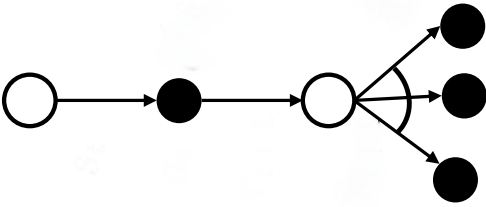
\includegraphics[width=0.2\textwidth]{dQ}
\caption[双Q-learning回溯图]{双Q-learning回溯图}
\end{figure}
%------------------------------------------------
\begin{myalgorithm}[双Q-learning]
\State 参数:步长$ \alpha \in (0,1] $,探索率$ \epsilon > 0 $
\State 初始化:$ \forall s \in S^+, a \in A(s) $,任意初始化$ q_1(s,a), q_2(s,a), q_1(\text{终止}, \cdot) = q_2(\text{终止}, \cdot) = 0 $
\For{每一幕}
\State 初始化$ s $
\While{$ s $不是终止状态}
\State 基于$ q_1 + q_2 $,使用$ \epsilon $-greedy策略在$ s $选择$ a $并执行,观察$ r, s' $
\If{以$ 0.5 $的概率}
\State $ q_1(s, a) \gets q_1(s, a) + \alpha [r + \gamma q_2(s', argmax_a Q_1(s',a)) - Q_1(s, a)] $
\Else
\State $ q_2(s, a) \gets q_2(s, a) + \alpha [r + \gamma q_1(s', argmax_a Q_2(s',a)) - Q_2(s, a)] $
\EndIf
\State $ s \gets s' $
\EndWhile
\EndFor
\end{myalgorithm}
%------------------------------------------------
\subsection[n-TD]{n-TD\tip{n-TD}}
n-TD作为MC和TD的一般推广,在两种极端方法间找到了性能更好的平衡点。n-TD在$ n $步后进行更新,截断得到$ n $步回报。
$$ G_{t:t + n} \doteq r_{t + 1} + \gamma r_{t + 2} + \dots + \gamma^{n - 1} r_{t + n} + \gamma^n v_{t + n - 1}(s_{t + n}) $$

其中$ v_{t + n}(s_t) \doteq v_{t + n - 1}(s_t) + \alpha[G_{t:t + n} - v_{t + n - 1}(s_t)] $。
%------------------------------------------------
\begin{myalgorithm}[n-TD]
\State 输入:待评估策略$ \pi $
\State 参数:步长$ \alpha \in (0,1], n \in N_+ $
\State 初始化:$ \forall s \in S $,任意初始化$ v(s) $
\For{每一幕}
\State 初始化$ s_0 $为非终止状态
\State $ T \gets \infty $
\For{$ t = 0, 1, 2, \dots $}
\If{$ t < T $}
\State 根据$ \pi(\cdot|s_t) $获得$ a_t $并执行,观察$ r_{t + 1}, s_{t + 1} $
\If{$ S_{t + 1} $是终止状态}
\State $ T \gets t + 1 $
\EndIf
\EndIf
\State $ \tau \gets t - n + 1 $ \Comment{$ \tau $是正在更新的状态的时间}
\If{$ \tau \geq 0 $}
\State $ G \gets \sum_{i = \tau + 1}^{\min(\tau + n,T)} \gamma^{i - \tau - 1}R_i $
\If{$ \tau + n < T $}
\State $ G \gets G + \gamma^n V(S_{\tau + n}) $
\EndIf
\State $ V(S_{\tau}) \gets V(S_{\tau}) + \alpha[G - V(S_{\tau})] $
\EndIf
\If{$ \tau = T - 1 $}
\State break
\EndIf
\EndFor
\EndFor
\end{myalgorithm}
%------------------------------------------------
\subsection[n-Sarsa]{n-Sarsa\tip{n-Sarsa}}
n-Sarsa统一了Sarsa和MC,其节点转移全部基于采样得到的单独路径:
$$ q_{t + n}(s_t, a_t) \doteq q_{t + n - 1}(s_t, a_t) + \alpha [G_{t:t + n} - q_{t + n - 1}(s_t, a_t)] $$

n-期望Sarsa只对最后一个状态到动作的转移展开:
$$ G_{t:t + n} \doteq r_{t + 1} + \gamma r_{t + 2} + \dots + \gamma^{n - 1} r_{t + n} + \gamma^n q_{\pi}(s_{t + n}, a_{t + n}) $$

\begin{figure}[H]
\centering
\subfloat[n-Sarsa]{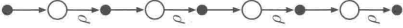
\includegraphics[width=.6\textwidth]{nSarsa}} \\
\subfloat[n-期望Sarsa]{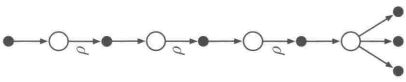
\includegraphics[width=.6\textwidth]{neSarsa}}
\caption[n-Sarsa回溯图]{n-Sarsa回溯图}
\end{figure}
%------------------------------------------------
\begin{myalgorithm}[n-Sarsa]
\State 参数:步长$ \alpha \in (0,1] $,探索率$ \epsilon > 0 $,步数$ n \in N_+ $
\State 初始化:$ \forall s \in S, a \in A $,任意初始化$ Q(s, a) $,初始化$ \pi $(如基于$ Q $的$ \epsilon $-greedy策略)
\For{每一幕}
\State 初始化$ s_0 $为非终止状态,根据$ \pi(\cdot|s_0) $选取$ a_0 $
\State $ T \gets \infty $
\For{$ t = 0, 1, 2, \dots $}
\If{$ t < T $}
\State 执行$ a_t $,观察$ r_{t + 1}, s_{t + 1} $
\If{$ s_{t + 1} $是终止状态}
\State $ T \gets t + 1 $
\Else
\State 根据$ \pi(\cdot|s_{t + 1}) $选取$ a_{t + 1} $
\EndIf
\EndIf
\State $ \tau \gets t - n + 1$ \Comment{$ \tau $是正在更新的状态的时间}
\If{$ \tau \geq 0 $}
\State $ G \gets \sum_{i = \tau + 1}^{\min(\tau + n,T)} \gamma^{i - \tau - 1}R_i $
\If{$ \tau + n < T $}
\State $ G \gets G + \gamma^n Q(s_{\tau + n}, a_{\tau + n}) $
\EndIf
\State $ Q(S_{\tau}, A_{\tau}) \gets Q(s_{\tau}, a_{\tau}) + \alpha[G - Q(s_{\tau}, a_{\tau})] $
\EndIf
\If{$ \tau = T - 1 $}
\State break
\EndIf
\EndFor
\EndFor
\end{myalgorithm}
%------------------------------------------------
\paragraph{off-policy-n-TD}
$$ v_{t + n}(s_t) \doteq v_{t + n - 1}(s_t) + \alpha \rho_{t:t + n - 1}[G_{t:t + n} - v_{t + n - 1}(s_t)] $$

其中重要度采样率为目标策略和行为策略采取$ n $个动作的相对概率:
$$ \rho_{t:h} \doteq \prod_{k = t}^{\min(h, T - 1)} \frac{\pi(a_k|s_k)}{b(a_k|s_k)} $$
%------------------------------------------------
\begin{myalgorithm}[n-期望Sarsa-off-policy]
\State 输入:$ b(a|s) > 0 $
\State 参数:步长$ \alpha \in (0,1] $,探索率$ \epsilon > 0 $,步数$ n \in N_+ $
\State 初始化:$ \forall s \in S, a \in A $,任意初始化$ Q(s, a) $,初始化$ \pi $
\For{每一幕}
\State 初始化$ s_0 $为非终止状态,根据$ b(\cdot|s_0) $选取$ a_0 $
\State $ T \gets \infty $
\For{$ t = 0, 1, 2, \dots $}
\If{$ t < T $}
\State 执行$ a_t $,观察$ r_{t + 1}, s_{t + 1} $
\If{$ s_{t + 1} $是终止状态}
\State $ T \gets t + 1 $
\Else
\State 根据 $ b(\cdot|s_{t + 1}) $选取$ a_{t + 1} $
\EndIf
\EndIf
\State $ \tau \gets t - n + 1 $ \Comment{$ \tau $是正在更新的状态的时间}
\If{$ \tau \geq 0 $}
\State $ \rho \gets \prod_{i = \tau + 1}^{\min(\tau + n - 1,T - 1)} \frac{\pi(A_i|S_i)}{b(A_i|S_i)}$ \Comment{重要性采样权重}
\State $ G \gets \sum_{i = \tau + 1}^{\min(\tau + n,T)} \gamma^{i - \tau - 1}R_i $
\If{$ \tau + n < T $}
\State $ G \gets G + \gamma^n \sum_a \pi(a|s_{\tau + n})Q(s_{\tau + n}, a)$ \Comment{期望Sarsa使用期望值}
\EndIf
\State $ Q(s_{\tau}, a_{\tau}) \gets Q(s_{\tau}, a_{\tau}) + \alpha \rho[G - Q(s_{\tau}, a_{\tau})] $
\EndIf
\If{$ \tau = T - 1 $}
\State break
\EndIf
\EndFor
\EndFor
\end{myalgorithm}
%------------------------------------------------
\subsection[对比与补充]{对比与补充}\label{sec:TD back}
Sarsa较为保守,在存在风险的任务中,会避开低回报动作; Q-learning较为乐观,更倾向于探索并找到最优解。在存在陷阱的任务中,Sarsa会比Q-learning取得更好的结果。

补充见\ref{sec:TD}。
%----------------------------------------------------------------------------------------
\section{表格型方法总结对比}\tip{表格型方法总结对比}
基于模型的方法(DP、启发式搜索)主要进行规划,无模型的方法(MC、TD)主要进行学习,二者的核心都是值函数的计算。
%------------------------------------------------
\paragraph{表格型方法介绍}\label{sec:table back}
见\ref{sec:table}
%------------------------------------------------
\paragraph{三个维度}
\begin{itemize}
\item 更新:期望更新能产生更好的估计,但是需要更多的计算。
\item 自举程度。
\item 同轨/离轨。
\end{itemize}

\begin{figure}[H]
\centering
\subfloat[总结对比]{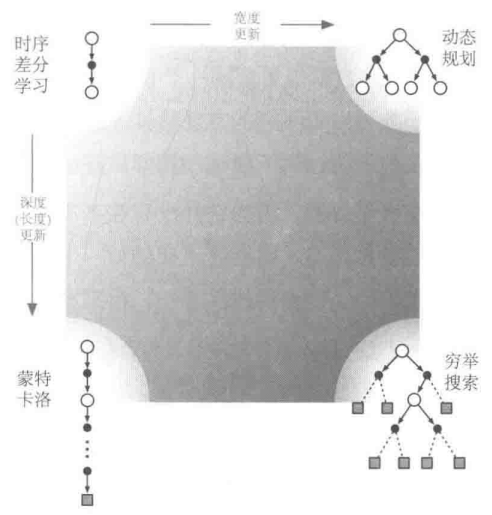
\includegraphics[width=.4\textwidth]{all}} \quad
\subfloat[更新对比]{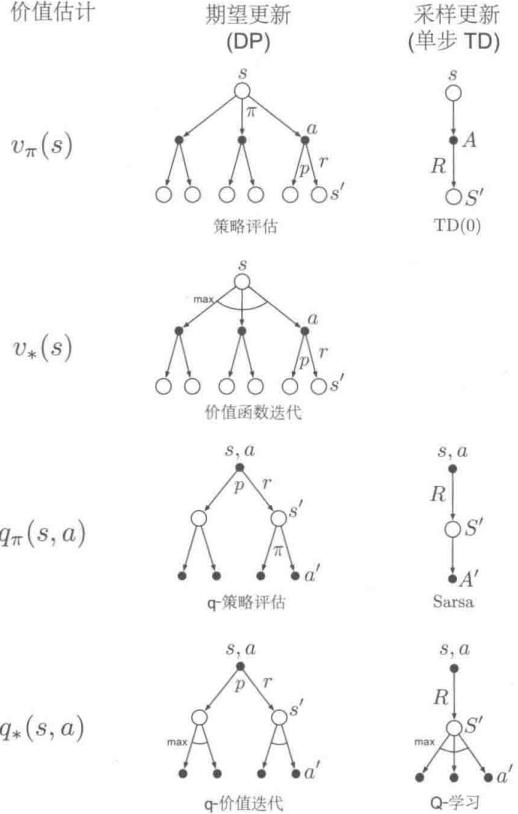
\includegraphics[width=.4\textwidth]{compare_update}} \\
\subfloat[DP表达式]{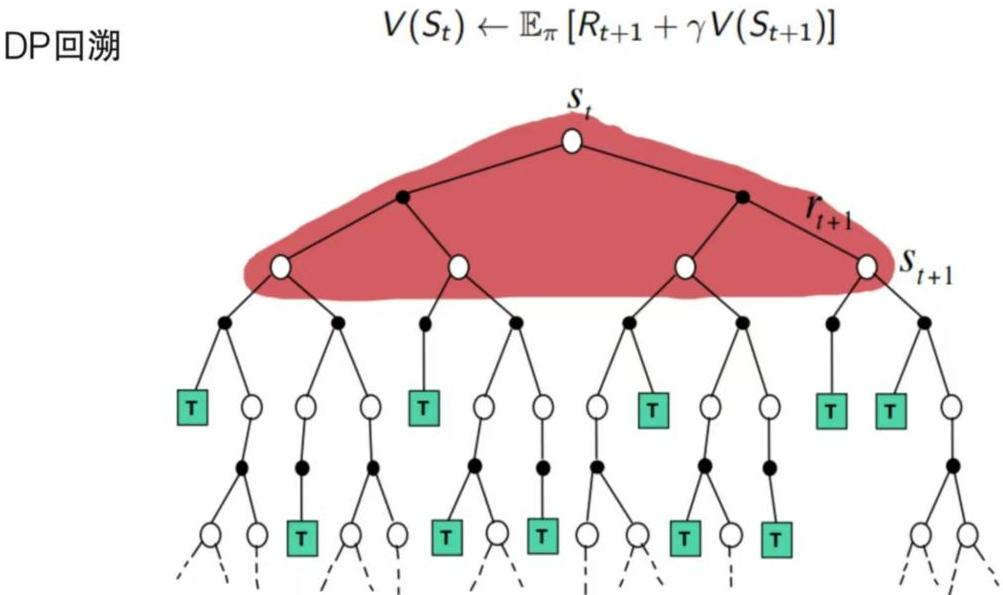
\includegraphics[width=.3\textwidth]{compare_DP}} \quad
\subfloat[MC表达式]{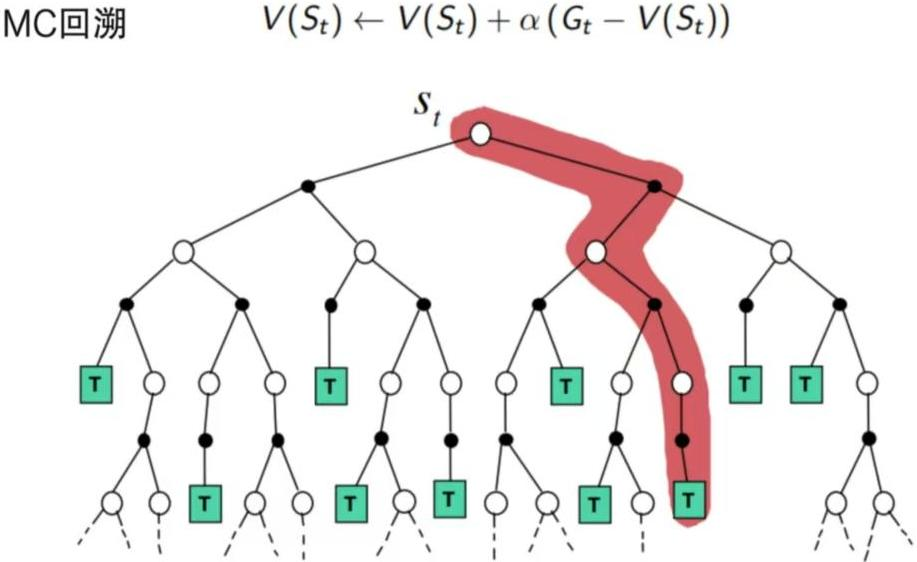
\includegraphics[width=.3\textwidth]{compare_MC}} \quad
\subfloat[TD表达式]{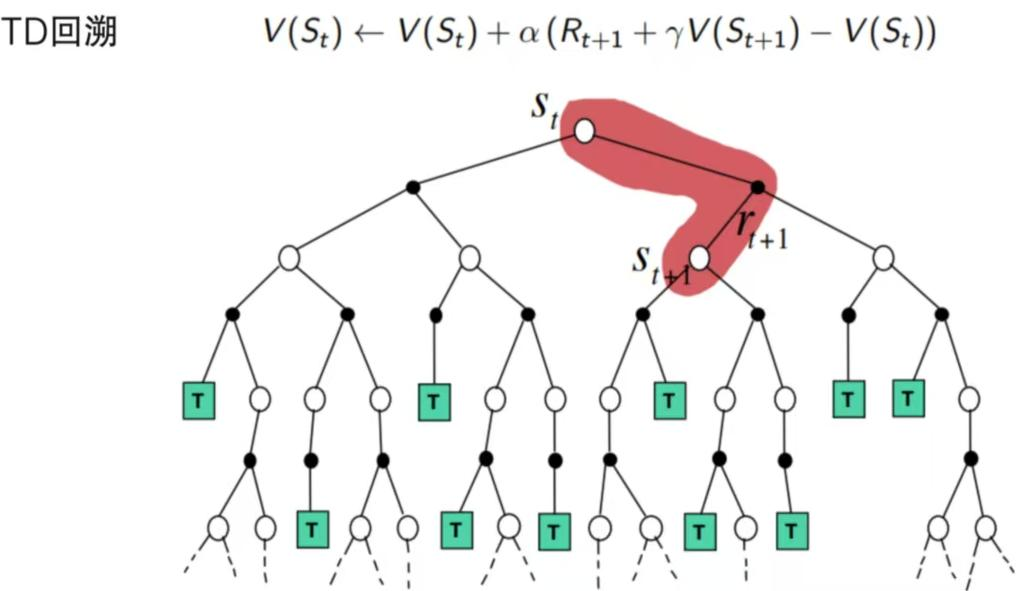
\includegraphics[width=.3\textwidth]{compare_TD}}
\caption[表格型方法对比]{表格型方法对比}
\end{figure}
%------------------------------------------------
\paragraph{表达式对比}
统一格式:
$$ q_{t + 1}(s_t, a_t) = q_t(s_t, a_t) + \alpha_t(s_t, a_t)[\bar{q}_t - q_t(s_t, a_t)] $$

\begin{table}[H]
\centering
\caption{各算法中的$ \bar{q}_t $表达式}
\begin{tabular}{|c|l|c|}
\hline
算法 & $ \bar{q}_t $表达式 & 求解目标 \\
\hline
Sarsa & $ r_{t + 1} + \gamma q_t(s_{t + 1}, a_{t + 1}) $ & \multirow{3}{*}{贝尔曼方程} \\
\cline{1-2}
n-Sarsa & $ r_{t + 1} + \gamma r_{t + 2} + \cdots + \gamma^n q_t(s_{t + n}, a_{t + n}) $ &  \\
\cline{1-2}
期望Sarsa & $ r_{t + 1} + \gamma \sum_{a \in A} \pi_t(a|s_{t + 1}) q_t(s_{t + 1}, a) $ &  \\
\hline
Q-learning & $ r_{t + 1} + \gamma \max_a q_t(s_{t + 1}, a) $ & 贝尔曼最优方程 \\
\hline
MC & $ r_{t + 1} + \gamma r_{t + 2} + \cdots $ & 贝尔曼方程 \\
\hline
\end{tabular}
\end{table}
%----------------------------------------------------------------------------------------
\section{值函数近似}
%------------------------------------------------
\subsection[值函数近似]{值函数近似\tip{值函数近似与随机梯度下降}}
$$ \hat{v}(s, \omega) \approx v_{\pi}(s), \omega \in R^d, d \ll |S| $$
%------------------------------------------------
\paragraph{目标函数}
$$ J(\omega) = E[(v_{\pi}(s) - \hat{v}(s, \omega))^2] $$

对$ s $按重要程度加权:
$$ \overline{VE}(\omega) \doteq \sum_{s \in S} \mu(s) [v_\pi(s) - \hat{v}(s, w)]^2 $$

一般无法保证最优,求解局部最优。
%------------------------------------------------
\paragraph{近似方法}\label{sec:kernal back}
\begin{itemize}
\item $ v_\pi(s_t) $:
\begin{itemize}
\item MC:$ G_t $。
\item TD:$ r_{t + 1} + \gamma \hat{v}(s_{t + 1}, \omega_t) $。
\end{itemize}
\item $ \hat{v}(s, \omega) $:
\begin{itemize}
\item 线性参数:$ \hat{v}(s, \omega) = \phi(s)^T \omega $,$ \phi(s) $为特征函数。
\begin{itemize}
\item 多项式基函数。
\item 傅里叶基函数$ \phi_i(s) = \cos(i \pi s), s \in [0, 1] $。
\item 径向基函数$ \phi_i(s) = e^{-\frac{||s - c_i||^2}{2\sigma_i^2}} $。
\item 表格法可视为特殊情况。
\end{itemize}
\item 非线性参数:
\begin{itemize}
\item 神经网络:输入状态,网络参数为$ \omega $,输出$ \hat{v}(s, \omega) $。
\item 决策树。
\item 模糊网络。
\end{itemize}
\item 非参数方法:核函数(见\ref{sec:kernal})、高斯回归等。
\end{itemize}
\end{itemize}
%------------------------------------------------
\paragraph{优势}
\begin{itemize}
\item 具有一定泛化能力,适应部分观测问题。
\item 曲线拟合:用少量参数储存状态,阶数越高越近似。
\end{itemize}
%------------------------------------------------
\subsection[随机梯度下降]{随机梯度下降(SGD)}
$$ \omega_{k + 1} = \omega_k - \alpha_k \nabla_\omega J(\omega_k) $$

其中,
\begin{align*}
\nabla_\omega J(\omega)
&= \nabla_\omega E[(v_\pi(s) - \hat{v}(s, \omega))^2] \\
&= E[\nabla_\omega (v_\pi(s) - \hat{v}(s, \omega))^2] (\text{有界可换求导与期望顺序}) \\
&= -2E[(v_\pi(s) - \hat{v}(s, \omega)) \nabla_\omega \hat{v}(s, \omega)]
\end{align*}

因此$ \omega_{k + 1} = \omega_k + \underbrace{\alpha}_{\text{步长}}[v_\pi(s_k) - \hat{v}(s_k, \omega_k)]\nabla_\omega \hat{v}(s_k, \omega_k) $。
%------------------------------------------------
\paragraph{负梯度方向降速最快}
梯度方向增长最快,负梯度方向下降最快。
%------------------------------------------------
\begin{myalgorithm}[梯度MC]
\State 输入:待评估$ \pi $,可微函数$ \hat{v}:S \times R^d \to R $
\State 参数:步长$ \alpha > 0 $
\State 初始化:任意初始化$ w \in R^d $
\Loop \Comment{对每一幕}
\State 根据$ \pi $生成一幕交互数据$ s_0, a_0, r_1, s_1, a_1, \cdots, r_T, s_T $
\For{$ t = 0, 1, \cdots, T - 1 $}
\State $ w_{t + 1} \gets w_t + \alpha_t[G_t - \hat{v}(s_t, w_t)]\nabla_{\omega} \hat{v}(s_t, w_t)$
\EndFor
\EndLoop
\end{myalgorithm}
%------------------------------------------------
\paragraph{半梯度下降}
只考虑$ w_t $对估计值的影响,而忽略对目标的影响。在使用自举目标时,目标本身依赖于$ w $,有偏。
\begin{itemize}
\item 优势:学习速度较快,支持持续在线学习,无需等待幕结束。
\item 局限:稳健性差,在非线性函数近似中可能不稳定。
\end{itemize}
%------------------------------------------------
\begin{myalgorithm}[半梯度TD($ 0 $)]
\State 输入:待评估$ \pi $,可微函数$ \hat{v}:S^+ \times R^d \to R, \hat{v}(\text{终止}, \cdot) = 0 $
\State 参数:步长$ \alpha > 0 $
\State 初始化:任意初始化$ w \in R^d $
\Loop \Comment{对每一幕}
\State 初始化$ s $
\For{$ t = 0, 1, \cdots, T - 1 $}
\State 选取$ a_t \sim \pi(\cdot|s_t) $并采取,观察$ r_t, s_{t + 1} $
\State $ w_{t + 1} \gets w_t + \alpha_t[r_{t + 1} + \gamma\hat{v}(s_{t + 1}, w_t) - \hat{v}(s_t, w_t)]\nabla_{\omega} \hat{v}(s_t, w_t) $
\If{$ s_{t + 1} $ 为终止状态}
\State break
\EndIf
\EndFor
\EndLoop
\end{myalgorithm}
%------------------------------------------------
\subsection[批方法]{批方法}
最小二乘法减少迭代计算量:
$$ LS(\omega) = \sum_{t = 1}^{T}[q_t^{\pi} - \hat{q}(s_t, a, \omega)]^2 = E_D[(q^{\pi} - \hat{q}(s, a, \omega))^2] $$
%------------------------------------------------
\subsection[DQN]{DQN(Deep Q-Network,深度Q网络)\tip{DQN}}
利用卷积神经网络作为非线性函数近似器,最小化损失函数,适用于高维空间:
$$ J(\omega) = E\{[R + \gamma \max_{a' \in A(S')} \hat{q}(S', a', \underbrace{\omega^-}_{\text{目标网络}}) - \hat{q}(S, A, \underbrace{\omega}_{\text{主网络}})]^2\} $$

目标网络:$ y^{DQN} = r + \gamma \max_{a'} Q(s', a'; \theta^-) $。
%------------------------------------------------
\paragraph{主要技术}
\begin{itemize}
\item 两个网络:主网络$ \hat{q}(s, a, \omega) $和目标网络$ \hat{q}(s', a', \omega^-) $,后者参数阶段性从前者同步。
\begin{itemize}
\item 防止过拟合:
\begin{itemize}
\item 随机丢弃法(dropout)。
\item 批量归一化(batch normalization)。
\item 残差直连边。
\end{itemize}
\item 更新:
\begin{itemize}
\item 软更新:部分更新。
\item 硬更新:直接复制。
\end{itemize}
\end{itemize}
\item 经验回放(Experience Replay)\tip{经验回放}:存储经验到固定大小的回放缓冲区,训练时从中随机选取。可以打乱样本相关性,提升训练稳定性。可改进为优先经验回放。
\item 帧堆叠:将图像作为神经网络输入时,堆叠多帧图像作为输入,并跳帧选取放入帧,增加时间信息。
\item 奖励裁剪(Reward Clipping):将奖励限制在特定范围内(甚至使用符号函数),避免大奖励幅度波动,提升训练稳定性,适用于奖励范围差异大的环境。
\end{itemize}
%------------------------------------------------
\begin{myalgorithm}[DQN]
\State 初始化:$ \omega, \omega^- $,经验回放缓冲区$ B = \{(s, a, r, s')\} $,计数器$ t \gets 0 $
\Loop
\If{$ t \mod C = 0 $} \Comment{每隔C步更新目标网络(初始化一致)}
\State $ \omega^- \gets \omega $
\EndIf
\State 从$ B $中均匀采样小批量样本$ \{(s, a, r, s')\} $
\For{每个样本}
\If{$ s' $ 是终止状态}
\State $ y \gets r $
\Else
\State $ y \gets r + \gamma \max_{a'} \hat{q}(s', a', \omega^-) $ \Comment{计算目标值}
\EndIf
\EndFor
\State 使用小批量样本$ \{(s, a, y)\} $更新主网络参数$ \omega $,最小化损失$ [y - \hat{q}(s, a, \omega)]^2 $
\State $ t \gets t + 1 $
\EndLoop
\end{myalgorithm}
%------------------------------------------------
\paragraph{double-DQN}
两个值函数逼近网络,一个选择动作,一个评估值函数。

目标网络:$ y^{DDQN} = r + \gamma Q[s', argmax_a Q(s_{t + 1}, a, \theta_t), \theta^-] $。
%----------------------------------------------------------------------------------------
\section[策略梯度]{策略梯度(policy gradient)}
%------------------------------------------------·
\subsection[概念]{概念\tip{策略梯度}}
将策略参数化,搜索策略空间,是同轨策略:
$$ \pi(a|s, \theta) = \pi_{\theta}(a|s) $$
%------------------------------------------------
\paragraph{梯度与梯度上升(倪推导)}~\\

学习$ \theta $使以下指标最大。
\begin{itemize}
\item 平均状态价值:
$$ \bar{v}_\pi = \sum_{s \in S} d(s) v_\pi(s) = E[v_\pi(S)] $$

其中$ d(s) \geq 0 $为$ s $的权重,$ \sum_{s \in S} d(s) = 1 $,其可由以下方法选取:
\begin{itemize}
\item 均匀分布:$ d(s) = \frac{1}{|S|} $。
\item 只关心$ s_0 $:$ d(s_0) = 1, d(s \neq s_0) = 0 $。
\item 平稳分布:$ d_{\pi}^T P_{\pi} = d_{\pi}^T $,根据访问频次赋予概率。
\end{itemize}
\item 平均单步奖励:
\begin{align*}
\bar{r}_\pi &= \sum_{s \in S} \underbrace{d_{\pi}(s)}_{\text{平稳分布}} \underbrace{r_\pi(s)}_{\sum_{a \in A} \pi(a|s)\underbrace{r(s, a)}_{\sum_{r \in R} r p(r|s, a)}} = E[r_\pi(S)] \\
&= \lim_{n \to \infty} \frac{1}{n}E[\sum_{k = 1}^{n} R_{t + k}] = \lim_{n \to \infty} \frac{1}{n}E[\sum_{k = 1}^{n} R_{t + k}|S_t = s_0]
\end{align*}
\end{itemize}

梯度为:
\begin{align*}
\nabla_\theta J(\theta) &= \sum_{s \in S} \eta(s) \sum_{a \in A} \nabla_\theta \pi(a|s, \theta) q_\pi(s, a) \\
&= \sum_{s \in S} \eta(s) \sum_{a \in A} \pi(a|s, \theta) \nabla_\theta \ln \pi(a|s, \theta) q_\pi(s, a) \\
&= E[\nabla_\theta \ln \pi(A|S, \theta) q_\pi(S, A)] \\
&\approx \nabla_\theta \ln \pi(a|s, \theta) q_\pi(s, a) (\text{采样近似})
\end{align*}

为确保$ \pi(a|s, \theta) > 0 $,使用softmax函数,$ \pi(a|s, \theta) = \frac{e^{h(s, a, \theta)}}{\sum_{a' \in A} e^{h(s, a', \theta)}} $。
\begin{align*}
\theta_{t + 1} &= \theta_t + \alpha\nabla_\theta J(\theta) = \theta_t + \alpha E[\nabla_\theta \ln \pi(A|S, \theta_t) q_\pi(S, A)] \\
&= \theta_t + \alpha \underbrace{\nabla_\theta \ln \pi(a_t|s_t, \theta_t)}_{\beta_t = \frac{q_\pi(s_t, a_t)}{\pi(a_t|s_t, \theta_t)}} \underbrace{q_\pi(s_t, a_t)}_{q(s_t, a_t)\text{近似}} (\text{随机梯度})
\end{align*}    

\begin{itemize}
\item $ \alpha\beta_t $足够小时,若$ \beta_t > 0 $,则选择$ (s_t, a_t) $的概率增加,且幅度与$ \beta_t $正相关。
\item $ \beta_t $与$ q_{\pi}(s_t, a_t) $正相关,与$ \pi(a_t|s_t, \theta_t) $负相关,倾向于选择高价值动作,探索低概率动作。
\end{itemize}
%------------------------------------------------
\paragraph{似然率策略梯度(郭推导)}~\\

记$ R(\tau) = \sum_{t = 0}^H R(s_t, u_t) $,目标函数为$ U(\theta) = \sum_{\tau} P(\tau, \theta) R(\tau) $,其梯度为:
\begin{align*}
\nabla_\theta U(\theta) &= \nabla_\theta \sum_{\tau} P(\tau, \theta) R(\tau) = \sum_{\tau} \nabla_\theta P(\tau, \theta) R(\tau) (\text{运算换序}) \\
&= \sum_{\tau} P(\tau, \theta) \frac{\nabla_\theta P(\tau, \theta)}{P(\tau, \theta)} R(\tau) = \sum_{\tau} P(\tau, \theta) \nabla_\theta \ln P(\tau, \theta) R(\tau) (\text{复合求导})
\end{align*}

经验平均为:
$$ \nabla_\theta U(\theta) \approx \hat{g} = \frac{1}{m} \sum_{i = 1}^m \nabla_\theta \ln P(\tau, \theta) R(\tau) $$

其无偏但方差很大,其中
\begin{align*}
\nabla_\theta\ln P(\tau^{(i)}, \theta) &= \nabla_\theta\ln[\prod_{t = 0}^{H} P(s_{t + 1}^{(i)}|s_t^{(i)}, u_t^{(i)}) \cdot \pi_\theta(u_t^{(i)}|s_t^{(i)})] \\
&= \nabla_\theta[\underbrace{\sum_{t = 0}^{H} \ln P(s_{t + 1}^{(i)}|s_t^{(i)}, u_t^{(i)})}_{\text{与动力学无关}} + \underbrace{\sum_{t = 0}^{H}\ln\pi_\theta(u_t^{(i)}|s_t^{(i)})}_{\text{只与策略相关}}] \\
&= \nabla_\theta[\sum_{t = 0}^{H} \ln\pi_\theta(u_t^{(i)}|s_t^{(i)})] = \underbrace{\sum_{t = 0}^{H} \nabla_\theta\ln\pi_\theta(u_t^{(i)}|s_t^{(i)})}_{\text{策略梯度}} 
\end{align*}

减小方差:
\begin{itemize}
\item 基线。
\item 修改值函数。
\end{itemize}
%------------------------------------------------
\paragraph{优势}
\begin{itemize}
\item 可以逼近确定性策略,可以逼近任意概率分布,不受$ q(s, a) $限制,策略是更简单的函数逼近。
\item 策略参数化更容易加入先验知识。
\item 在状态空间大时,存储和泛化能力强。
\end{itemize}
%------------------------------------------------·
\subsection[REINFORCE]{REINFORCE(MC-policy gradient)\tip{REINFORCE}}
用MC估计$ q_\pi(s, a) $,使用与$ \theta $无关的$ G_t $代替$ q_\pi(s_t, a_t) $:
$$ \theta_{t + 1} \doteq \theta_t + \alpha G_t \nabla_{\theta} ln \pi (a_t|s_t, \theta_t) $$
%------------------------------------------------·
\begin{myalgorithm}[REINFORCE]
\State 输入:可微分的$ \pi(a|s, \theta) $
\State 参数:步长$ \alpha > 0 $,折扣因子$ \gamma \in (0, 1) $
\State 初始化:初始化$ \theta \in R^{d'} $
\Loop
\State 按照$ \pi(\cdot|\cdot, \theta) $生成一幕$ s_0, a_0, r_1, \cdots, s_{T - 1}, a_{T - 1}, r_T $
\For{$ t = 0, 1, \cdots, T - 1 $}
\State $ G_t \gets \sum_{k = t + 1}^{T} \gamma^{k - t - 1}R_k $
\State $ \theta \gets \theta + \alpha G_t \nabla_{\theta} \ln \pi(a_t|s_t, \theta_t) $
\EndFor
\EndLoop
\end{myalgorithm}
%----------------------------------------------------------------------------------------
\section{Actor-Critic方法}
%------------------------------------------------·
\subsection[概念]{概念\tip{Actor-Critic方法}}
结合策略梯度和价值方法。
$$ \theta_{t + 1} = \theta_t + \alpha \nabla_\theta \ln \pi(a_t|s_t, \theta_t) q_\pi(s_t, a_t) $$
\begin{itemize}
\item 演员(Actor):策略更新,用于采取行动,对应算法更新。
\item 评论家(Critic):策略评估或价值估计,用于评判策略,对应估计$ q_{\pi}(s, a) $,采用TD方法。
\end{itemize}
%------------------------------------------------·
\begin{myalgorithm}[QAC]
\State 初始化:策略参数$ \theta $和评论家参数$ w $
\For{每个回合}
\For{$ t = 0, 1, 2, \ldots, T - 1 $}
\State 根据$ \pi(a|s_t, \theta_t) $选择$ a_t $,观察$ r_{t + 1}, s_{t + 1} $,再根据$ \pi(a|s_{t + 1}, \theta_t) $选择$ a_{t + 1} $
\State $ \delta_t = r_{t + 1} + \gamma q(s_{t + 1}, a_{t + 1}, w_t) - q(s_t, a_t, w_t) $ \Comment{TD误差}
\State $ w_{t + 1} = w_t + \alpha_w \delta_t \nabla_w q(s_t, a_t, w_t) $ \Comment{评论家价值更新}
\State $ \theta_{t + 1} = \theta_t + \alpha_\theta \nabla_\theta \ln \pi(a_t|s_t, \theta_t) q(s_t, a_t, w_{t + 1}) $ \Comment{演员策略更新}
\EndFor
\EndFor
\end{myalgorithm}
%------------------------------------------------·
\subsection[基线优势]{基线优势\tip{基线优势}}
基本的Actor-Critic方法有较大方差,引入基线降低。
%------------------------------------------------
\paragraph{基线}
$$ \nabla_\theta J(\theta) = E_{S \sim \eta, A \sim \pi}\{\nabla_\theta \ln \pi(A|S, \theta_t) [q_\pi(S, A) - b(S)]\} $$

策略梯度期望不变:
\begin{align*}
E_{S\sim\eta,A\sim\pi}[\nabla_\theta\ln\pi(A|S,\theta_t)b(S)] &= \sum_{s \in S} \eta(s) \sum_{a \in A} \nabla_\theta\pi(a|s,\theta_t)b(s) \\
&= \sum_{s \in S} \eta(s) b(s) \sum_{a\in A} \nabla_\theta\pi(a|s,\theta_t) \\
&= \sum_{s \in S} \eta(s) b(s) \nabla_\theta 1 (\text{交换求和与求导}) \\
&= 0
\end{align*}

为使策略梯度方差最小化,求偏导得:
\begin{align*}
b^*(s) &= \frac{E_{A\sim\pi}[||\nabla_\theta\ln\pi(A|s,\theta_t)||^2 q_\pi(s,A)]}{E_{A\sim\pi}[||\nabla_\theta\ln\pi(A|s,\theta_t)||^2]} \\
&= E_{A\sim\pi}[q_\pi(s,A)] (\text{省略权重}) \\
&= v_{\pi}(s)
\end{align*}

如果直接用$ b(s) = q_{\pi}(s, a) $,会导致策略梯度为$ 0 $。
%------------------------------------------------
\paragraph{优势函数}
$$ \theta_{t + 1} = \theta_t + \alpha E\{\nabla_\theta \ln \pi(A|S, \theta_t) \underbrace{[q_\pi(S, A) - v_{\pi}(s)]}_{\text{优势函数}\delta_{\pi}(S, A)}\} $$

此时,$ \beta_t = \frac{\delta_{\pi}(s_t, s_t)}{\pi(a_t|s_t, \theta_t)} $,正相关项为相对值,而非绝对值,更合理。

使用TD进行近似:
$$ \delta_t = q_t(s_t, a_t) - v_t(s_t) \approx r_{t + 1} + \gamma v_t(s_{t + 1}) - v_t(s_t) $$

这时只需要一个网络进行估计。
%------------------------------------------------
\begin{myalgorithm}[A2C]
\State 初始化:策略参数$ \theta $和评论家参数$ w $
\For{每个回合}
\For{$ t = 0, 1, 2, \ldots, T - 1 $}
\State 根据$ \pi(a|s_t, \theta_t) $选择$ a_t $,执行后观察$ r_{t + 1}, s_{t + 1} $
\State $ \delta_t = r_{t + 1} + \gamma v(s_{t + 1}, w_t) - v(s_t, w_t) $ \Comment{优势函数}
\State $ w_{t + 1} = w_t + \alpha_w \delta_t \nabla_w v(s_t, w_t) $ \Comment{评论家价值更新}
\State $ \theta_{t + 1} = \theta_t + \alpha_\theta \delta_t \nabla_\theta \ln \pi(a_t|s_t, \theta_t) $ \Comment{演员策略更新}
\EndFor
\EndFor
\end{myalgorithm}
%------------------------------------------------
\paragraph{off-policy}
加入重要性采样由on-policy变成off-policy:
$$ \nabla_\theta J(\theta) = E_{S \sim \rho, A \sim \beta}[\frac{\pi(A|S,\theta)}{\beta(A|S)}\nabla_\theta\ln\pi(A|S,\theta)q_\pi(S,A)] $$

其中$ \beta $是行为策略,$ \rho $是状态分布。其也可以采用上述基线$ b^*(s) $。
%------------------------------------------------·
\begin{myalgorithm}[重要性采样离轨Actor-Critic]
\State 初始化:$ \beta(a|s), \pi(a|s,\theta_0), v(s,w_0) $
\For{每个回合}
\For{$ t = 0, 1, 2, \ldots, T - 1 $}
\State 根据$ \beta(s_t) $选择$ a_t $,观察$ r_{t + 1}, s_{t + 1} $。
\State $ \delta_t = r_{t + 1} + \gamma v(s_{t + 1}, w_t) - v(s_t, w_t) $ \Comment{优势函数}
\State $ w_{t + 1} = w_t + \alpha_w \frac{\pi(a_t|s_t,\theta_t)}{\beta(a_t|s_t)} \delta_t \nabla_w v(s_t, w_t) $ \Comment{评论家价值更新}
\State $ \theta_{t + 1} = \theta_t + \alpha_\theta \frac{\pi(a_t|s_t,\theta_t)}{\beta(a_t|s_t)} \delta_t \nabla_\theta \ln \pi(a_t|s_t, \theta_t) $ \Comment{演员策略更新}
\EndFor
\EndFor
\end{myalgorithm}
%------------------------------------------------·
\subsection[TRPO与PPO]{TRPO与PPO\tip{TRPO与PPO}}
%------------------------------------------------·
\subsubsection[TRPO]{TRPO(Trust Region Policy Optimization,信赖域策略优化)}
限制每次策略更新的幅度,保证稳定性和单调提升。
%------------------------------------------------
\paragraph{替代回报函数}
\begin{align*}
\eta(\tilde{\pi}) &= \eta(\pi) + \underbrace{E_{s_0, a_0, \cdots \sim \tilde{\pi}}[\sum_{t = 0}^{\infty} \gamma^t A_{\pi}(s_t, a_t)]}_{\text{新旧策略回报差}} \\
&= \eta(\pi) + \sum_{s} \rho_{\tilde{\pi}}(s) \sum_{a} \tilde{\pi}(a|s) A^{\pi}(s, a) \\
L_{\pi}(\tilde{\pi}) &= \eta(\pi) + \sum_{s} \textcolor{red}{\rho_{\pi}(s)} \sum_{a} \tilde{\pi}(a|s) A^{\pi}(s, a) (\text{忽略状态分布变化}) \\
&= \eta(\pi) + E_{s \sim \rho_{\theta_{old}}, a \sim \pi_{\theta_{old}}}[\frac{\tilde{\pi}_{\theta}(a|s)}{\pi_{\theta_{old}}(a|s)} A_{\theta_{old}}(s, a)] (\text{重要性采样动作分布})
\end{align*}

有$ L_{\pi_{\theta_{old}}}(\pi_{\theta_{old}}) = \eta(\pi_{\theta_{old}}), \nabla_{\theta} L_{\pi_{\theta_{old}}}(\pi_{\theta}) \big|_{\theta = \theta_{old}} = \nabla_{\theta} \eta(\pi_{\theta}) \big|_{\theta = \theta_{old}} $。

令$ \alpha = D^{\max}_{TV}(\pi, \tilde{\pi}), \epsilon = \max_{s, a}|A_{\pi}(s, a)|$,惩罚因子$ C = \frac{2\epsilon\gamma}{(1 - \gamma)^2} $,则有:
$$ \eta(\tilde{\pi}) \geq L_{\pi}(\tilde{\pi}) - \frac{4\epsilon}{(1 - \gamma)^2} \alpha^2 \quad \eta(\tilde{\pi}) \geq L_{\pi}(\tilde{\pi}) - C D^{\max}_{KL}(\pi, \tilde{\pi}) $$
%------------------------------------------------
\paragraph{优化:共轭梯度搜索}
问题转化为:
\begin{align*}
&\max_{\theta}[L_{\theta_{old}}(\theta) - C D^{\max}_{KL}(\theta_{old}, \theta)] \\
\overset{\text{迭代步长较小}}{\Longrightarrow} 
&\max_{\theta} E_{s \sim \rho_{\theta_{old}}, a \sim \pi_{\theta_{old}}}[\frac{\pi_{\theta}(a|s)}{\pi_{\theta_{old}}(a|s)} A_{\theta_{old}}(s, a)], \quad D^{\max}_{KL}(\theta_{old}, \theta) \leq \delta \\
\underset{\text{平均KL散度}}{\overset{\text{策略状态空间分布}}{\Longrightarrow}}
&\max_{\theta} E_{s \sim \textcolor{red}{\pi_{\theta_{old}}}, a \sim \pi_{\theta_{old}}}[\frac{\pi_{\theta}(a|s)}{\pi_{\theta_{old}}(a|s)} A_{\theta_{old}}(s, a)], \quad E_{s \sim \pi_{\theta_{old}}}\{D_{KL}[\pi_{\theta_{old}}(\cdot|s)\pi_{\theta}(\cdot|s)]\} \leq \delta \\
\underset{\text{约束二次逼近}}{\overset{\text{目标线性逼近}}{\Longrightarrow}}
&\max_{\theta}[\nabla_{\theta} L_{\theta_{old}}(\theta) \big|_{\theta = \theta_{old}} \cdot (\theta - \theta_{old})], \quad \frac{1}{2}(\theta_{old} - \theta)^T \underbrace{A(\theta_{old})}_{Fisher \text{信息矩阵}} (\theta_{old} - \theta) \leq \delta
\end{align*}
%------------------------------------------------·
\subsubsection[PPO]{PPO(Proximal Policy Optimization,近端策略优化)}
限制新旧策略的变化幅度,保证策略更新的稳定性,简化TRPO的实现并提升效率。
\begin{align*}
L^{CLIP}(\theta) &= E_t[\min\{r_t(\theta) \hat{A}_t, clip[r_t(\theta), 1 - \epsilon, 1 + \epsilon]\hat{A}_t\}] \\
L_t^{CLIP + VF + S}(\theta) &= \hat{E}_t\{L_t^{CLIP}(\theta) - c_1 L_t^{VF}(\theta) + c_2 S[\pi_\theta](s_t)\}
\end{align*}

其中,
\begin{itemize}
\item 值函数损失函数$ L_t^{VF} $。
\item 熵$ S $。
\item 优势函数估计$ \hat{A}_t = \delta_t + (\gamma\lambda)\delta_{t + 1} + \dots + (\gamma\lambda)^{T - t + 1}\delta_{T - 1} $,$ \delta $为TD误差。
\end{itemize}
%------------------------------------------------·
\begin{myalgorithm}[PPO]
\State 初始化$ \theta, \theta_{old} $
\For{每个回合}
\For{$ actor = 1, 2, \ldots, N $}
\State 用$ \pi_{\theta_{old}} $采集$ T $步序列$ \{(s_t, a_t, r_t, s_{t + 1})\}_{t = 1}^T $
\State 优势估计$ \hat{A}_t $
\State 回报$ \hat{R}_t $
\EndFor
\State 汇总所有样本,数量为$ NT $
\For{$ k = 1, 2, \ldots, K $}
\State 随机采样$ M $个minibatch
\State 概率比$ r_t(\theta) = \frac{\pi_\theta(a_t|s_t)}{\pi_{\theta_{old}}(a_t|s_t)} $
\State clip损失:$ L^{CLIP} = \min(r_t(\theta)\hat{A}_t, clip(r_t(\theta), 1 - \epsilon, 1 + \epsilon)\hat{A}_t) $
\State 值函数损失$ L^{VF} $和熵正则项$ S[\pi_\theta](s_t) $
\State 总损失$ L = E[L^{CLIP} - c_1 L^{VF} + c_2 S] $
\State 对$ \theta $梯度下降优化$ L $
\EndFor
\State $ \theta_{old} \gets \theta $
\EndFor
\end{myalgorithm}
%------------------------------------------------·
\subsection[确定性策略Actor-Critic方法]{确定性策略Actor-Critic方法}
%------------------------------------------------·
\subsubsection[DPG]{DPG}
在策略是确定性时,有off-policy方法:
$$ \nabla_\theta J(\theta) = \sum_{s \in S} \underbrace{\rho_\mu(s)}_{\text{状态分布}} \nabla_\theta \mu(s)[\nabla_a q_\mu(s, a)]\bigg|_{a = \mu(s)} = E_{S \sim \rho_\mu}\{\nabla_\theta \mu(S)[\nabla_a q_\mu(S, a)]\bigg|_{a =\mu(S)}\} $$
%------------------------------------------------·
\begin{myalgorithm}[确定性策略Actor-Critic(DPG)]
\State 初始化:$ \beta(a|s), \mu(s, \theta_0), q(s, a, w_0) $。\Comment{$ \beta $可用$ \mu $+噪声替代}
\For{每个回合}
\For{$ t = 0, 1, 2, \ldots, T - 1 $}
\State 根据$ \beta(s_t) $生成$ a_t $,观察$ r_{t + 1}, s_{t + 1} $
\State $ \delta_t = r_{t + 1} + \gamma q(s_{t + 1}, \mu(s_{t + 1}, \theta_t), w_t) - q(s_t, a_t, w_t) $ \Comment{优势函数}
\State $ w_{t + 1} = w_t + \alpha_w \delta_t \nabla_w q(s_t, a_t, w_t) $ \Comment{评论家价值更新}
\State $ \theta_{t + 1} = \theta_t + \alpha_\theta \nabla_\theta \mu(s_t, \theta_t)[\nabla_a q(s_t, a, w_{t + 1})]|_{a = \mu(s_t)} $ \Comment{演员策略更新}
\EndFor
\EndFor
\end{myalgorithm}
%------------------------------------------------·
\subsubsection[DDPG]{DDPG\tip{DDPG}}
结合DQN和DPG,演员、评论家各有主网络和目标网络,一共四个网络。为在确定性策略中保障探索性,引入噪声。
%------------------------------------------------
\paragraph{OU(Ornstein-Uhlenbeck)噪声}~\\

均值回归随机过程$ dX_t = \underbrace{\theta}_{\text{回归速度参数}}(\underbrace{\mu}_{\text{长期均值}} - X_t)dt + \underbrace{\sigma}_{\text{噪声强度}} \underbrace{dW_t}_{\text{维纳过程}} $,离散为:
$$ X_{t + 1} = X_t + \theta(\mu - X_t) + \sigma \epsilon_t $$
\begin{itemize}
\item 相邻时刻噪声值相关,适合连续控制任务,使动作平滑变化。
\item 噪声逐渐回归均值,避免长期偏离,提供了自然的探索衰减机制。
\end{itemize}
%------------------------------------------------
\begin{myalgorithm}[DDPG]
\State 初始化:随机初始化评论家网络$ Q(s, a|\theta^Q) $和演员网络$ \mu(s|\theta^\mu) $,初始化目标网络$ Q', \mu' $,使$ \theta^{Q'} \gets \theta^Q, \theta^{\mu'} \gets \theta^\mu $,初始化经验回放池$ R $
\For{每个回合}
\State 初始化探索噪声过程$ N $
\State 接收初始状态$ s_1 $
\For{$ t = 1, \dots, T $}
\State 选择$ a_t = \mu(s_t|\theta^\mu) + N_t $ \Comment{带噪声的确定性策略}
\State 执行$ a_t $,观察$ r_t, s_{t + 1} $
\State 存储转移$ (s_t, a_t, r_t, s_{t + 1}) $到$ R $ \Comment{经验回放}
\State 从$ R $中随机采样$ N $个小批量$ (s_i, a_i, r_i, s_{i + 1}) $
\State 目标值$ y_i = r_i + \gamma Q'(s_{i + 1}, \mu'(s_{i + 1}|\theta^{\mu'})|\theta^{Q'}) $ \Comment{目标网络}
\State 更新评论家:最小化损失$ L = \frac{1}{N}\sum_i (y_i - Q(s_i, a_i|\theta^Q))^2 $
\State 更新演员:$\nabla_{\theta^\mu} J \approx \frac{1}{N} \sum_i \nabla_a Q(s, a|\theta^Q)|_{s = s_i, a = \mu(s_i)} \nabla_{\theta^\mu} \mu(s|\theta^\mu)|_{s_i} $
\State 软更新目标网络参数
\EndFor
\EndFor
\end{myalgorithm}
%----------------------------------------------------------------------------------------
\section{策略搜索方法总结对比}\tip{策略搜索方法总结对比}
$$
\text{策略搜索方法} \begin{cases} 
\text{无模型} \begin{cases} 
\text{随机策略} \begin{cases} 
\text{策略梯度:TRPO} \\ \text{统计学习} \\ \text{路径积分} \end{cases} \\ 
\text{确定性策略:DDPG} \\ \text{EM方法} \\ \text{粒子滤波方法} \end{cases} \\ 
\text{基于模型:指导策略搜索(GPS),传统控制器+监督学习} \end{cases}
$$
%----------------------------------------------------------------------------------------
\section{多智能体强化学习}\tip{多智能体强化学习}
%------------------------------------------------
\subsection[概念]{概念}
\begin{minipage}{0.3\textwidth}
\paragraph{分类}
\begin{itemize}
\item 完全协作。
\item 完全竞争。
\item 混合策略。
\end{itemize}
\end{minipage}
\hfill
\begin{minipage}{0.6\textwidth}
\paragraph{挑战}
\begin{itemize}
\item 单智能体视角下,其它智能体是动态的,值函数为相互依赖的联合值函数。
\item 智能体间存在博弈关系,求均衡解。
\end{itemize}
\end{minipage}
%------------------------------------------------
\paragraph{博弈论}
\begin{itemize}
\item 参与人行动先后顺序:
\begin{itemize}
\item 静态博弈:同时行动。
\item 动态博弈:有先后行动顺序,常用博弈树拓展表述。
\end{itemize}
\item 参与人知识储备:
\begin{itemize}
\item 完美信息博弈:已知相关信息。
\item 非完美信息博弈:不完全知道相关信息。
\end{itemize}
\end{itemize}
%------------------------------------------------
\paragraph{完美信息静态博弈的纳什均衡策略(Nash equilibrium)}
所有智能体以最佳策略应对,全理性,没有智能体能单独偏离自身策略来改善自身回报。所有智能体采取纳什均衡策略应比部分智能体采取纳什均衡策略的价值高。
%------------------------------------------------
\paragraph{非完美信息博弈的扩展式博弈}
七元组$ \{H, Z, P, p, u, I ,\sigma_c\} $,分别是当前节点已知所有信息(包含个人私有信息),终止状态集合,玩家集合,非终止状态到玩家映射,非终止状态到实数映射,终止状态到实数映射(玩家到终止状态时获得的回报),信息集,策略。
%------------------------------------------------
\subsection[算法]{算法}
\begin{figure}[H]
\centering
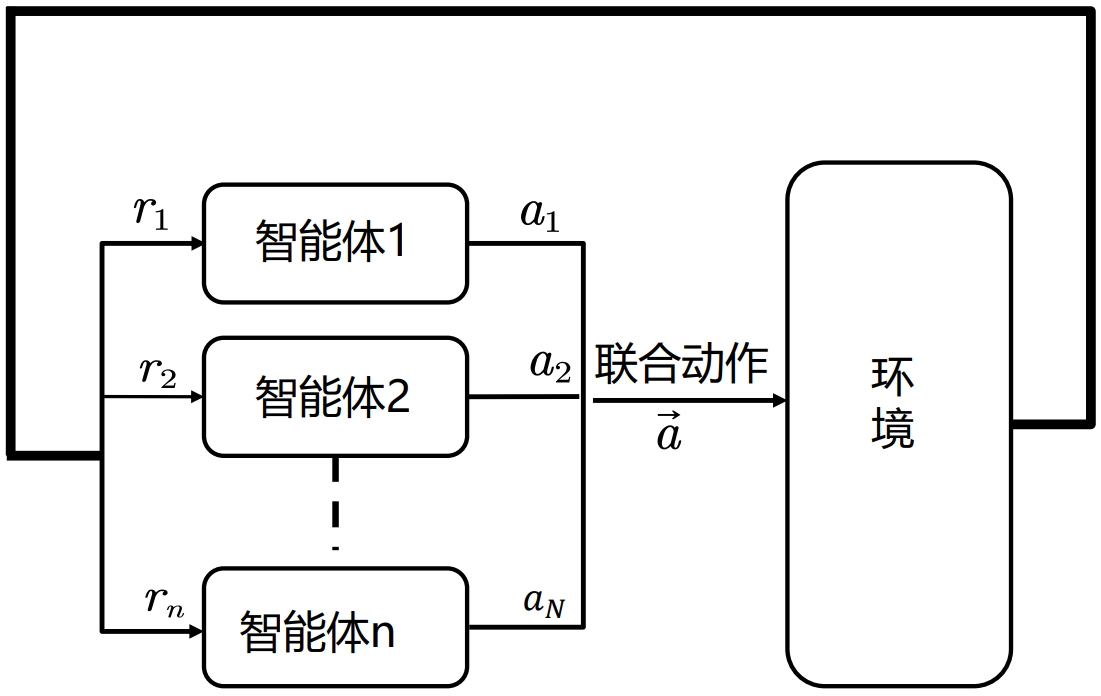
\includegraphics[width=0.4\textwidth]{many}
\caption[多智能体强化学习]{多智能体强化学习}
\end{figure}

\begin{itemize}
\item 完全协作。
\item 完全竞争:MinimaxQ-learning算法。
\item 混合策略:纳什Q-learning算法,Friend-or-foe Q-learning算法,wolf策略爬山算法。
\item 基于微分对策略。
\item 深度强化学习算法。
\end{itemize}
%----------------------------------------------------------------------------------------
\section{附录}
%------------------------------------------------
\subsection[概念与原理]{概念与原理}
%------------------------------------------------
\subsubsection[历史与发展]{历史与发展}\label{sec:history}
\begin{enumerate}
\item 源于动物学习心理学的试错法:效应定律(Edward Thorndike),条件反射(巴普洛夫),快乐-痛苦系统(图灵),向“老师”学习到向“评论家”学习,自动学习机(M.L.Tsetlin),分类器系统(救火队算法和遗传算法)。
\item 最优控制:贝尔曼方程与马尔可夫决策过程(Richard Bellman),维度灾难。
\item 时序差分方法:次级强化物,广义强化(Klopf),与试错法结合(actor-critic方法,Sutton),与最优控制结合(Q-learning,Chris Watkins)。
\end{enumerate}

返回正文\ref{sec:history back}。
%------------------------------------------------
\subsubsection[贝尔曼最优方程求解]{贝尔曼最优方程求解}\label{sec:Scalability Mapping}
%------------------------------------------------
\paragraph{收缩映射定理}
若$ f(x) $是收缩映射,则存在唯一一个不动点$ x^* $满足$ f(x^*) = x^* $。针对$ x_{k + 1} = f(x_k) $,在$ x_k \to x^*, k \to \infty $的过程中,收敛速度成指数级增长。
\begin{itemize}
\item 存在性:$ ||x_{k + 1} - x_k|| = ||f(x_{k + 1}) - f(x_k)|| \leq \gamma||x_k - x_{k - 1}|| \leq \dots \leq \gamma^k||x_1 - x_0|| \overset{\gamma < 1, \gamma^k \to 0}{\Longrightarrow} x_{k + 1} - x_k \to 0 $。同理可得$ ||x_m - x_n|| \leq \frac{\gamma^n}{1 - \gamma}||x_1 - x_0|| \to 0 $,进而得到$ \{x_k\} $是收敛数列,存在$ \lim_{k \to \infty} x_k = x^* $。
\item 唯一性:$ ||f(x_k) - x_k|| = ||x_{k + 1} - x_k|| $,其快速收敛到$ 0 $,则在极限处有不动点$ f(x^*) = x^* $。假设存在另一不动点,其必与该不动点相等。
\item 指数级收敛:$ ||x^* - x_n|| = \lim_{m \to \infty}||x_m - x_n|| \leq \frac{\gamma^n}{1 - \gamma}||x_1 - x_0|| \to 0 $。
\end{itemize}
%------------------------------------------------
\paragraph{贝尔曼最优方程的伸缩映射性}~\\

$ \forall v1,v2 $,有贝尔曼最优方程$ \pi_i^* \doteq \arg \max_{\pi}(r_\pi + \gamma P_\pi v_i) $,

故$ f(v_i) = \max_{\pi}(r_\pi + \gamma P_\pi v_i) = r_{\pi_i^*} + \gamma P_{\pi_i^*} v_i \geq r_{\pi_j^*} + \gamma P_{\pi_j^*} v_i (i \neq j) $,则
\begin{align*}
f(v_1) - f(v_2) 
&= r_{\pi_1^*} + \gamma P_{\pi_1^*} v_1 - (r_{\pi_2^*} + \gamma P_{\pi_2^*} v_2) \\
&\leq r_{\pi_1^*} + \gamma P_{\pi_1^*} v_1 - (r_{\pi_1^*} + \gamma P_{\pi_1^*} v_2) \\
&= \gamma P_{\pi_1^*} (v_1 - v_2)
\end{align*}

同理有$ f(v_2) - f(v_1) \leq \gamma P_{\pi_2^*} (v_2 - v_1) $,故$ \gamma P_{\pi_2^*} (v_1 - v_2)\leq f(v_1) - f(v_2) \leq \gamma P_{\pi_1^*} (v_1 - v_2) $,

取边界极值$ z $,有$ |f(v_1) - f(v_2)| \leq z $,即$ ||f(v_1) - f(v_2)||_\infty \leq ||z||_\infty $。

又有$ ||z||_\infty = max_i |z_i| \leq \gamma ||v_1 - v_2||_\infty $,所以$ ||f(v_1) - f(v_2)||_\infty \leq \gamma ||v_1 - v_2||_\infty $。
%------------------------------------------------
\paragraph{贝尔曼最优方程解的性质}
\begin{itemize}
\item 唯一性:唯一解$ v^* $能通过$ v_{k + 1} = f(v_k) = \max_{\pi \in \Pi} (r_\pi + \gamma P_\pi v_k) $迭代求解,其对应策略$ \pi^* = argmax_{\pi \in \Pi}(r_\pi + \gamma P_\pi v^*) $。
\item 最优性($ v^* = v_{\pi^*} \geq v_{\pi} $):由$ v_{\pi} = r_{\pi} + \gamma P_{\pi} v_{\pi} $和$ v^* = \max_{\pi}(r_{\pi} + \gamma P_{\pi} v^*) = r_{\pi^*} + \gamma P_{\pi^*} v^* \geq r_{\pi} + \gamma P_{\pi} v^* $,可得$ v^* - v_{\pi} \geq (r_{\pi} + \gamma P_{\pi} v^*) - (r_{\pi} + \gamma P_{\pi} v_{\pi}) = \gamma P_{\pi}(v^* - v_{\pi}) $,即有$ v^* - v_{\pi} \geq \gamma P_{\pi}(v^* - v_{\pi}) \geq \dots \geq \gamma^n P_{\pi}^n(v^* - v_{\pi}) $,由于$ \gamma < 0 $,$ \forall p_{ij} \in P_{\pi}, p_{ij} \leq 1 $,$ \lim_{n \to \infty} \gamma^n P_{\pi}^n(v^* - v_{\pi}) $趋于$ 0 $,所以$ v^* \geq v_{\pi} $。
\end{itemize}

返回正文\ref{sec:Scalability Mapping back}。
%------------------------------------------------
\subsection[表格型方法]{表格型方法}
%------------------------------------------------
\subsubsection[DP补充]{DP补充}\label{sec:DP}
\begin{enumerate}
\item 异步动态规划:使用任意可用状态值,以任意顺序更新,避免遍历更新,减小计算量。
\item 广义策略迭代(GPI):策略评估和策略改进以更细粒度进行交替,可视为竞争与合作。
\item 效率:DP的时间复杂度是动作与状态数量的多项式级,在面对维度灾难时,优于线性规划和直接搜索。
\end{enumerate}

返回正文\ref{sec:DP back}。
%------------------------------------------------
\subsubsection[MC补充]{MC补充}
%------------------------------------------------
\paragraph{减小重要性采样的方差}\label{sec:MC}
\begin{itemize}
\item 折扣敏感:把$ \gamma $视作幕终止的概率,得到第$ n $步终止的无折扣部分回报$ \sum_{i = 1}^n R_{t + i} $,即平价部分回报。全回报$ G_t = \sum_{i = 1}^{T - t} \gamma^{i - 1}R_{t + i} $可视为各平价部分回报的加权和,即该步截止得到的回报与概率之积的和。适用于普通型和加权型。
\item 每次决策型:$ E[\rho_{t:T - 1}G_t] = E[\tilde{G_t}] = E[\sum_{i = 1}^{T - t} \gamma^{i - 1} \rho_{t:t + i - 1}R_{t + i}] $。适用于普通型。
\end{itemize}

返回正文\ref{sec:MC back}。
%------------------------------------------------
\subsubsection[TD补充]{TD补充}\label{sec:TD}
%------------------------------------------------
\paragraph{改进方法}
\begin{itemize}
\item 批量更新:值函数根据增量和改变,在处理整批数据后才更新。
\item 最大化偏差:贪心策略和柔性策略都在隐式估计最大值,会产生正偏差,致使回报值偏离,带来明显错误决策。
\item 后位状态:利用先验知识,知晓动作后状态,并有后位值函数。在后位状态相同的时候可以迁移,减少计算量。
\end{itemize}
%------------------------------------------------
\paragraph{带控制变量的每次决策模型}~\\

为保证不被选择的动作不会因$ \rho_t = 0 $而回报为$ 0 $,使方差较大,采取以下n步回报off-policy方法:
$$ G_{t:h} \doteq \rho_t (r_{t + 1} + \gamma G_{t + 1:h}) + \underbrace{(1 - \rho_t) v_{h - 1}(s_t)}_{\text{控制变量}} $$

其中控制变量保证$ \rho_t = 0 $时估计值不收缩,且不改变更新期望。

可写为以下递归形式:
\begin{align*}
G_{t:h} 
&\doteq r_{t + 1} + \gamma[\rho_{t + 1} G_{t + 1:h} + \bar{v}_{h - 1}(s_{t + 1}) - \rho_{t + 1} Q_{h - 1}(s_{t + 1}, a_{t + 1})] \\
&= r_{t + 1} + \gamma \rho_{t + 1}[G_{t + 1:h} - Q_{h - 1}(s_{t + 1}, a_{t + 1})] + \gamma \bar{v}_{h - 1}(s_{t + 1})
\end{align*}
%------------------------------------------------
\paragraph{树回溯}~\\

树回溯不使用重要度采样,缓解了off-policy因所学内容相关性小比on-policy慢的问题。相比以沿途收益和底部节点估计值为更新目标的算法,树回溯的更新源于整个树的行为值估计,即各叶子节点的行为值估计按出现概率加权。

单步回溯树:
$$ G_{t:t + 1} \doteq r_{t + 1} + \gamma \sum_{a} \pi(a|s_{t + 1}) Q_t(s_{t + 1}, a) $$

n-回溯树(递归形式),其对路径可能分支进行展开,不进行采样:
$$ G_{t:t + n} \doteq r_{t + 1} + \gamma \sum_{a \neq a_{t + 1}} \pi(a|s_{t + 1}) Q_{t + n - 1}(s_{t + 1}, a) + \gamma \pi(a_{t + 1}|s_{t + 1}) G_{t + 1:t + n} $$

\begin{figure}[H]
\centering
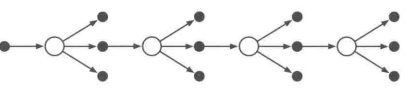
\includegraphics[width=0.6\textwidth]{ntree}
\caption[n-树回溯回溯图]{n-树回溯回溯图}
\end{figure}
%------------------------------------------------
\begin{myalgorithm}[n-树回溯]
\State 参数:步长$ \alpha \in (0,1], n \in N_+ $
\State 初始化:$ \forall s \in S, a \in A $,任意初始化$ Q(s, a) $,初始化$ \pi $
\For{每一幕}
\State 初始化$ s_0 $为非终止状态,根据它任意选取$ a_0 $
\State $ T \gets \infty $
\For{$ t = 0, 1, 2, \dots $}
\If{$ t < T $}
\State 执行$ a_t $,观察$ r_{t + 1}, s_{t + 1} $
\If{$ s_{t + 1} $是终止状态}
\State $ T \gets t + 1 $
\Else
\State 根据$ s_{t + 1} $选取$ a_{t + 1} $
\EndIf
\EndIf
\State $ \tau \gets t - n + 1 $ \Comment{$ \tau $是正在更新的状态的时间}
\If{$ \tau \geq 0 $}
\If{$ t + 1 \geq T $}
\State $ G \gets r_T $ 
\Else
\State $ G \gets r_{t + 1} + \gamma \sum_a \pi(a|s_{t + 1})Q(s_{t + 1}, a) $
\EndIf
\For{$ k = \min(t, T - 1) $递减到$ \tau + 1 $}
\State $ G \gets r_k + \gamma \sum_{a \neq a_k} \pi(a|s_k)Q(s_k,a) + \gamma \pi(a_k|s_k)G $
\EndFor
\State $ Q(s_{\tau}, a_{\tau}) \gets Q(s_{\tau}, a_{\tau}) + \alpha[G - Q(s_{\tau}, a_{\tau})] $
\EndIf
\If{$ \tau = T - 1 $}
\State break
\EndIf
\EndFor
\EndFor
\end{myalgorithm}
%------------------------------------------------
\paragraph{n-Q($ \sigma $)}
结合采样的Sarsa和展开的树回溯,在每个状态由参数$ \sigma $决定是采样还是展开,将两种线性情况组合起来:
$$ G_{t:h} \doteq r_{t + 1} + \gamma [\sigma_{t + 1}\rho_{t + 1} + (1 - \sigma_{t + 1})\pi(a_{t + 1}|s_{t + 1})][G_{t + 1:h} - Q_{h - 1}(s_{t + 1}, a_{t + 1})] + \gamma \bar{v}_{h - 1}(s_{t + 1}) $$

\begin{figure}[H]
\centering
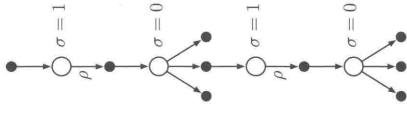
\includegraphics[width=0.6\textwidth]{Qsigma}
\caption[Q(sigma)回溯图]{Q(sigma)回溯图}
\end{figure}
%------------------------------------------------
\begin{myalgorithm}[n-Q($ \sigma $)-off-policy]
\State 输入:$ b(a|s) > 0 $
\State 参数:步长$ \alpha \in (0,1] $,探索率$ \epsilon > 0 $,步数$ n \in N_+ $
\State 初始化:$ \forall s \in S, a \in A $,任意初始化$ Q(s, a) $,初始化$ \pi $
\For{每一幕}
\State 初始化$ s_0 $为非终止状态
\State 根据$ b(\cdot|s_0) $选取$ a_0 $
\State $ T \gets \infty $
\For{$ t = 0, 1, 2, \dots $}
\If{$ t < T $}
\State 执行$ a_t $,观察$ r_{t + 1}, s_{t + 1} $
\If{$ s_{t + 1} $是终止状态}
\State $ T \gets t + 1 $
\Else
\State 根据$ b(\cdot|s_{t + 1}) $选取$ a_{t + 1} $
\State 选择$ \sigma_{t + 1} $ \Comment{指示是采样还是展开}
\State $ \rho_{t + 1} \gets \frac{\pi(a_{t + 1}|s_{t + 1})}{b(a_{t + 1}|s_{t + 1})}$ \Comment{重要性采样比率}
\EndIf
\EndIf
\State $ \tau \gets t - n + 1 $ \Comment{$ \tau $是正在更新的状态的时间}
\If{$ \tau \geq 0 $}
\State $ G \gets 0 $
\For{$ k = \min(t, T - 1) $递减到$ \tau + 1 $}
\If{$ k = T $}
\State $ G \gets r_T $
\Else
\State $ \bar{V} \gets \sum_a \pi(a|s_k)Q(s_k, a) $ \Comment{计算期望状态值}
\State $ G \gets r_k + \gamma[\sigma_k \rho_k + (1 - \sigma_k)\pi(a_k|s_k)][G - Q(s_k, a_k)] + \gamma\bar{v} $
\EndIf
\EndFor
\State $ Q(S_{\tau},A_{\tau}) \gets Q(s_{\tau}, a_{\tau}) + \alpha[G - Q(s_{\tau}, a_{\tau})] $
\EndIf
\If{$ \tau = T - 1 $}
\State break
\EndIf
\EndFor
\EndFor
\end{myalgorithm}

返回正文\ref{sec:TD back}。
%------------------------------------------------
\subsubsection[模型和规划]{模型和规划}\label{sec:table}
%------------------------------------------------
\paragraph{模型}
\begin{itemize}
\item 分布模型:生成所有可能的结果的描述与概率分布。
\item 样本模型:从所有可能中按概率分布采样一个确定结果。可由分布模型生成,一般更容易获得。
\end{itemize}
%------------------------------------------------
\paragraph{规划}
\begin{itemize}
\item 规划:以环境模型为输入,生成或改进与其交互的策略。
\item 规划空间:
\begin{itemize}
\item 状态空间规划:在状态空间搜索最优策略。
\item 方案空间规划:进化算法、偏序规划。
\end{itemize}
\item 规划时间:
\begin{itemize}
\item 后台规划:从环境模型生成模拟经验,改进策略或值函数。
\item 决策时规划:使用模拟经验为状态选择动作。
\end{itemize}
\end{itemize}
%------------------------------------------------
\paragraph{统一的状态空间规划算法}
通过仿真经验的回溯操作计算值函数,进而改进策略。
$$ \text{模型} \Longrightarrow \text{模拟经验} \overset{\text{回溯}}{\Longrightarrow} \text{值函数} \Longrightarrow \text{策略} $$
%------------------------------------------------
\subsubsection[Dyna-Q]{Dyna-Q}
学习和规划由相同算法完成,真实经验用于学习,模拟经验用于规划。
%------------------------------------------------
\begin{myalgorithm}[Dyna-Q]
\State 初始化:$ \forall s \in S, a \in A(S) $,初始化$ Q(s, a) $和$ Model(s, a) $
\Loop
\State $ s \gets $ 当前(非终止)状态 \Comment{学习}
\State 基于$ (s, Q) $选取$ a $,执行后观察$ r,s' $ \Comment{可用$ \epsilon $-greedy策略}
\State $ Q(s, a) \gets Q(s, a) + \alpha[r + \gamma \max_a Q(s', a) - Q(s, a)] $ \Comment{直接强化学习更新}
\State $ Model(s, a) \gets r,s' $
\For{$ i = 1,\dots,n $} \Comment{规划}
\State 随机选择已观测过的$ s $和其下采取过的$ a $
\State $ r,s' \gets Model(s, a) $ \Comment{从模型获取预测}
\State $ Q(s, a) \gets Q(s, a) + \alpha[r + \gamma \max_a Q(s', a) - Q(s, a)] $ \Comment{规划更新}
\EndFor
\EndLoop
\end{myalgorithm}
%------------------------------------------------
\subsubsection[改进方法]{改进方法}
鼓励长期未出现动作,模型可能不正确,需规避在次优解收敛。
%------------------------------------------------
\paragraph{优先遍历}
集中更新有收益动作,而非均匀采样。

关联前导动作和前导状态,在后续动作有收益时先更新前导动作价值,进行有效更新。按照价值改变多少对状态-动作对进行优先级排序,并由后至前反向传播出高影响序列。
%------------------------------------------------
\begin{myalgorithm}[确定性环境下的优先遍历]
\State 初始化:$ \forall s \in S, a \in A(s) $,初始化$ Q(s, a), Model(s, a) $,初始化优先级队列$ PQueue = NULL $
\Loop
\State $ s \gets $当前(非终止)状态
\State 基于$ (s, q) $选取$ a $,执行后观察$ r,s' $ \Comment{可用$ \epsilon $-greedy策略}
\State $ Model(s, a) \gets r,s'$
\State $ P \gets |r + \gamma \max_a Q(s', a) - Q(s, a)| $ \Comment{优先级}
\If{$ P > 0 $}
\State 将$ (s, a) $以优先级$ P $插入$ PQueue $
\EndIf
\For{$ i = 1, \dots, n $}
\If{$ PQueue = NULL $}
\State break
\EndIf
\State $ (s, a) \gets PQueue(0) $ \Comment{最高优先级}
\State $ r, s' \gets Model(s, a) $ \Comment{从模型获取预测}
\State $ Q(s, a) \gets Q(s, a) + \alpha[r + \gamma \max_a Q(s', a) - Q(s, a)] $ \Comment{规划更新}
\For{每个可达到$ s $的$ (\bar{s}, \bar{a}) $} \Comment{反向传播更新}
\State $ \bar{r}, \bar{s'} \gets Model(\bar{s}, \bar{a}) $
\If{$ \bar{s'} = s $}
\State $ P \gets |\bar{r} + \gamma \max_a Q(s, a) - Q(\bar{s}, \bar{a})| $
\If{$ P > 0 $}
\State 将$ (\bar{s}, \bar{a}) $以优先级$ P $插入$ PQueue $
\EndIf
\EndIf
\EndFor
\EndFor
\EndLoop
\end{myalgorithm}
%------------------------------------------------
\paragraph{on-policy轨迹采样}
借助模拟生成经验回溯更新,能跳过无关状态,获得最优部分策略。实时动态规划(RTDP)是其异步值迭代版本,可在较少访问频率下找到最优策略,并且产生轨迹所用的策略也会接近最优策略。
%------------------------------------------------
\paragraph{启发式搜索}
聚焦于当前状态。
%------------------------------------------------
\paragraph{预演算法}
作为MC的特例,通过平均多个起始于可能动作并遵循给定策略的模拟轨迹的回报来估计行为值。蒙特卡洛树搜索(MCTS)通过累积蒙特卡洛值估计来不断优化模拟轨迹的收益。

返回正文\ref{sec:table back}。
%------------------------------------------------
\subsection[值函数近似]{值函数近似}
%------------------------------------------------
\paragraph[核函数]{核函数}\label{sec:kernal}
\begin{itemize}
\item 基于记忆样本,使用RBF核,存储样本状态。核函数$ k(s, s') $可表示为特征向量$ x(s) $的内积,每个特征对应一个样本状态:
$$ k(s, s') = x(s)^T x(s') $$
\item 非参数化,不需要学习参数。
\item 避免高维计算,高效处理特征。
\item 线性参数化方法皆可重塑为核函数,相同训练数据下会得到近似结果。
\end{itemize}

返回正文\ref{sec:kernal back}。
%------------------------------------------------
\subsection[数学基础]{数学基础}
%------------------------------------------------
\paragraph{概率空间$ (\Omega, F, P) $}
\begin{itemize}
\item 性质
\begin{itemize}
\item 非负性:$ \forall A \in F, P(A) \geq 0 $。
\item 规范性:$ P(\Omega) = 1 $。
\item 可列可加性:若$ A_1, A_2, \dots $互斥,则$ P(\bigcup_{i = 1}^{\infty} A_i) = \sum_{i = 1}^{\infty} P(A_i) $。
\end{itemize}
\item 运算
\begin{itemize}
\item 补集:$ P(A^c) = 1 - P(A) $。
\item 交集:$ P(A \cap B) = P(A) + P(B) - P(A \cup B) $。
\end{itemize}
\end{itemize}
%------------------------------------------------
\paragraph{随机变量}
\begin{itemize}
\item 离散型
\begin{itemize}
\item 概率质量函数(PMF):$ P(X = x) = p(x), \sum_{x} p(x) = 1 $。
\item 期望:$ E[X] = \sum_{x} x p(x) $。
\end{itemize}
\item 连续型
\begin{itemize}
\item 概率密度函数(PDF):$ f(x) \geq 0, \int_{-\infty}^{\infty} f(x) dx = 1 $。
\item 期望:$ E[X] = \int_{-\infty}^{\infty} x f(x) dx $。
\end{itemize}
\item 方差:$ Var(X) = E[(X - E[X])^2] $。
\end{itemize}
%------------------------------------------------
\paragraph{条件概率与独立性}
\begin{itemize}
\item 条件概率:$ P(B|A) = \frac{P(A \cap B)}{P(A)}, P(A) > 0 $。
\item 全概率公式:$ P(B) = \sum_{A \subseteq F} P(B|A) P(A) $。
\item 贝叶斯定理:$ P(A|B) = \frac{P(B|A) P(A)}{P(B)} $。
\item 独立性: $ A,B $独立$ \iff $$ P(A \cap B) = P(A)P(B) $。
\item 条件独立:$ P(A ,B|C) = P(A|C)P(B|C) $。
\end{itemize}
%------------------------------------------------
\paragraph{大数定律与中心极限定理}
\begin{itemize}
\item 弱大数律:$ \frac{1}{n} \sum_{i = 1}^n X_i \overset{p}{\Longrightarrow} E[X] $。
\item 强大数律:$ \frac{1}{n} \sum_{i = 1}^n X_i \overset{a.s.}{\Longrightarrow} E[X] $。
\item 中心极限定理:$ X_1, X_2, \dots $独立同分布,均值为$ \mu $,方差为$ \sigma^2 < \infty $,则$ \frac{1}{\sqrt{n}} \sum_{i = 1}^n (X_i - \mu) \overset{d}{\Longrightarrow} N(0, \sigma^2) $。
\end{itemize}
%------------------------------------------------
\paragraph{泛函分析}
\begin{itemize}
\item 期望的线性:$ E[aX + bY] = a E[X] + b E[Y] $。
\item 协方差:$ Cov(X, Y) = E[(X - \mu_X)(Y - \mu_Y)] = E[XY] - \mu_X \mu_Y $。
\item 相关系数:$ \rho(X, Y) = \frac{Cov(X, Y)}{\sigma_X \sigma_Y} $。
\end{itemize}
%------------------------------------------------
\paragraph{状态分布}
\begin{itemize}
\item 均匀分布(各状态同等重要):$ J(\omega) = \frac{1}{|S|}\sum_{s \in S} [v_{\pi}(s) - \hat{v}(s, \omega)]^2 $。
\item 平稳分布(马氏过程长期行为):$ J(\omega) = \sum_{s \in S} d_{\pi}(s)[v_{\pi}(s) - \hat{v}(s, \omega)]^2 $。
\end{itemize}
%------------------------------------------------
\paragraph{信息论}
\begin{itemize}
\item 熵:不确定度的度量。
\begin{itemize}
\item 二值熵:$ H = -p \log(p) - (1 - p)\log(1 - p) $。
\item 交叉熵:$ H(P, Q) = -E_{P(x)} Q(x) = -\int P(x) \log Q(x) dx $。
\end{itemize}
\item KL散度:衡量两个概率分布之间的距离。
$$ D_{KL}(P||Q) = E_{x \sim P}[\log \frac{P(x)}{Q(x)}] = \int P(x) \log P(x) dx - \int P(x) \log Q(x) dx $$
\end{itemize}
%----------------------------------------------------------------------------------------
\end{document}